% Template for Elsevier CRC journal article
% version 1.2 dated 09 May 2011

% This file (c) 2009-2011 Elsevier Ltd.  Modifications may be freely made,
% provided the edited file is saved under a different name

% This file contains modifications for Procedia Computer Science

% Changes since version 1.1
% - added "procedia" option compliant with ecrc.sty version 1.2a
%   (makes the layout approximately the same as the Word CRC template)
% - added example for generating copyright line in abstract

%-----------------------------------------------------------------------------------
%% This template uses the elsarticle.cls document class and the extension package ecrc.sty
%% For full documentation on usage of elsarticle.cls, consult the documentation "elsdoc.pdf"
%% Further resources available at http://www.elsevier.com/latex

%-----------------------------------------------------------------------------------

%%%%%%%%%%%%%%%%%%%%%%%%%%%%%%%%%%%%%%%%%%%%%%%%%%%%%%%%%%%%%%
%%%%%%%%%%%%%%%%%%%%%%%%%%%%%%%%%%%%%%%%%%%%%%%%%%%%%%%%%%%%%%
%%                                                          %%
%% Important note on usage                                  %%
%% -----------------------                                  %%
%% This file should normally be compiled with PDFLaTeX      %%
%% Using standard LaTeX should work but may produce clashes %%
%%                                                          %%
%%%%%%%%%%%%%%%%%%%%%%%%%%%%%%%%%%%%%%%%%%%%%%%%%%%%%%%%%%%%%%
%%%%%%%%%%%%%%%%%%%%%%%%%%%%%%%%%%%%%%%%%%%%%%%%%%%%%%%%%%%%%%

%% The '3p' and 'times' class options of elsarticle are used for Elsevier CRC
%% The 'procedia' option causes ecrc to approximate to the Word template
\documentclass[3p,times,procedia]{elsarticle}
\flushbottom

%% The `ecrc' package must be called to make the CRC functionality available
\usepackage{ecrc}
\usepackage{amsmath}
\usepackage{amssymb}
\usepackage[bookmarks=false]{hyperref}
    \hypersetup{colorlinks,
      linkcolor=blue,
      citecolor=blue,
      urlcolor=blue}
%\usepackage{amsmath}


%% The ecrc package defines commands needed for running heads and logos.
%% For running heads, you can set the journal name, the volume, the starting page and the authors

%% set the volume if you know. Otherwise `00'
\volume{00}

%% set the starting page if not 1
\firstpage{1}

%% Give the name of the journal
\journalname{Procedia Computer Science}

%% Give the author list to appear in the running head
%% Example \runauth{C.V. Radhakrishnan et al.}
\runauth{P K Sangameswar}

%% The choice of journal logo is determined by the \jid and \jnltitlelogo commands.
%% A user-supplied logo with the name <\jid>logo.pdf will be inserted if present.
%% e.g. if \jid{yspmi} the system will look for a file yspmilogo.pdf
%% Otherwise the content of \jnltitlelogo will be set between horizontal lines as a default logo

%% Give the abbreviation of the Journal.
\jid{procs}

%% Give a short journal name for the dummy logo (if needed)
%\jnltitlelogo{Computer Science}

%% Hereafter the template follows `elsarticle'.
%% For more details see the existing template files elsarticle-template-harv.tex and elsarticle-template-num.tex.

%% Elsevier CRC generally uses a numbered reference style
%% For this, the conventions of elsarticle-template-num.tex should be followed (included below)
%% If using BibTeX, use the style file elsarticle-num.bst

%% End of ecrc-specific commands
%%%%%%%%%%%%%%%%%%%%%%%%%%%%%%%%%%%%%%%%%%%%%%%%%%%%%%%%%%%%%%%%%%%%%%%%%%

%% amssymb is already loaded above (with amsmath), so it is not repeated here.
%% The amsthm package provides extended theorem environments
%% \usepackage{amsthm}

%% The lineno packages adds line numbers. Start line numbering with
%% \begin{linenumbers}, end it with \end{linenumbers}. Or switch it on
%% for the whole article with \linenumbers after \end{frontmatter}.
%% \usepackage{lineno}

%% natbib.sty is loaded by default. However, natbib options can be
%% provided with \biboptions{...} command. Following options are
%% valid:

%%   round  -  round parentheses are used (default)
%%   square -  square brackets are used   [option]
%%   curly  -  curly braces are used      {option}
%%   angle  -  angle brackets are used    <option>
%%   semicolon  -  multiple citations separated by semi-colon
%%   colon  - same as semicolon, an earlier confusion
%%   comma  -  separated by comma
%%   numbers-  selects numerical citations
%%   super  -  numerical citations as superscripts
%%   sort   -  sorts multiple citations according to order in ref. list
%%   sort&compress   -  like sort, but also compresses numerical citations
%%   compress - compresses without sorting
%%
%% \biboptions{authoryear}

% \biboptions{}

% --- ecrc.sty bug workaround -------------------------------------------------
% ecrc.sty reads \abovelistskip<N>/\belowlistskip<N> via \csname but never
% defines them, so every list raises "Missing number"/"Illegal unit of measure".
% The errors are recoverable (LaTeX substitutes 0pt), so we define them as 0pt
% to silence the errors while leaving list spacing exactly as it renders today.
\newskip\abovelistskipi   \abovelistskipi=0pt
\newskip\belowlistskipi   \belowlistskipi=0pt
\newskip\abovelistskipii  \abovelistskipii=0pt
\newskip\belowlistskipii  \belowlistskipii=0pt
% -----------------------------------------------------------------------------

% if you have landscape tables
\usepackage[figuresright]{rotating}
% booktabs provides \toprule/\midrule/\bottomrule/\addlinespace used in Table 1
\usepackage{booktabs}
\usepackage{multirow}
% algorithm float + pseudocode (used by the dropout-aware training algorithm)
\usepackage{algorithm}
\usepackage{algpseudocode}
% --- Float placement: stop wide table* floats drifting into later sections.
%     dblfloatfix fixes double-column (table*/figure*) ordering and enables
%     bottom placement; the fractions let larger floats sit at page tops near
%     their definition instead of being deferred pages away. ---
\usepackage{dblfloatfix}
\renewcommand{\topfraction}{0.9}
\renewcommand{\bottomfraction}{0.8}
\renewcommand{\textfraction}{0.07}
\renewcommand{\floatpagefraction}{0.75}
\renewcommand{\dbltopfraction}{0.9}
\renewcommand{\dblfloatpagefraction}{0.75}
\setcounter{topnumber}{3}
\setcounter{bottomnumber}{2}
\setcounter{totalnumber}{5}
\setcounter{dbltopnumber}{3}
%\usepackage{harvard}
% put your own definitions here:
% Symbols for the related-work comparison table (Table 1)
\newcommand{\yes}{\checkmark}
\newcommand{\no}{\ensuremath{-}}
\newcommand{\pt}{\ensuremath{\sim}}
%   \newcommand{\cZ}{\cal{Z}}
%   \newtheorem{def}{Definition}[section]
%   ...

% add words to TeX's hyphenation exception list
%\hyphenation{author another created financial paper re-commend-ed Post-Script}

% declarations for front matter


\begin{document}
\begin{frontmatter}

%% Title, authors and addresses

%% use the tnoteref command within \title for footnotes;
%% use the tnotetext command for the associated footnote;
%% use the fnref command within \author or \address for footnotes;
%% use the fntext command for the associated footnote;
%% use the corref command within \author for corresponding author footnotes;
%% use the cortext command for the associated footnote;
%% use the ead command for the email address,
%% and the form \ead[url] for the home page:
%%
%% \title{Title\tnoteref{label1}}
%% \tnotetext[label1]{}
%% \author{Name\corref{cor1}\fnref{label2}}
%% \ead{email address}
%% \ead[url]{home page}
%% \fntext[label2]{}
%% \cortext[cor1]{}
%% \address{Address\fnref{label3}}
%% \fntext[label3]{}

\dochead{International Conference on Machine Learning and Data Engineering}%%%
%% Use \dochead if there is an article header, e.g. \dochead{Short communication}
%% \dochead can also be used to include a conference title, if directed by the editors
%% e.g. \dochead{17th International Conference on Dynamical Processes in Excited States of Solids}

%\title{%%Robustness of Spatio-temporal Graph Neural Networks to Sensor Dropout in Fault Localization for Partially Observable Distribution Grids%%

\title{Dropout-Aware Training for Sensor-Robust Fault Localization with Spatio-Temporal Graph Neural Networks}

%% use optional labels to link authors explicitly to addresses:
%% \author[label1,label2]{<author name>}
%% \address[label1]{<address>}
%% \address[label2]{<address>}



\author[1]{P K Sangameswar}
\author[1]{M Anbazhagan\corref{cor1}}
\ead{m\_anbazhagan@cb.amrita.edu}

\address[1]{Department of Computer Science and Engineering, Amrita School of Computing, Coimbatore, Amrita Vishwa Vidyapeetham, India}
% \address[b]{Department of Computer Science and Engineering, Amrita School of Computing, Amrita Vishwa Vidyapeetham, Coimbatore, Tamil Nadu, India}

\begin{abstract}
%% Text of abstract
Spatio-temporal graph neural networks (STGNNs) localize faults accurately in distribution grids instrumented with only a few micro-phasor measurement units ($\mu$PMUs), but their evaluations assume every sensor always reports, which deployed systems do not guarantee. Following the STGNN methodology of Karabulut et al.\ (2026) on the IEEE 123-bus feeder, we train five architectures on our own dataset, the strongest reaching a soft-voting macro-F1 of $0.85$, and present what is to our knowledge the first systematic evaluation of STGNN robustness to $\mu$PMU loss, dropping $k \in \{0,1,2,5,10\}$ of 25 sensors at inference. Within the architectures evaluated here, clean accuracy predicts robustness poorly: the most accurate one degrades the fastest, falling below $0.10$ at 40\% loss. Dropout-aware training, which masks measurement nodes during training, raises retention at 40\% loss from $5.7\%$ to $80.3\%$ on that backbone ($p<0.01$, paired over three training seeds) at measured parity in inference latency and parameter count, and improves all five architectures. An availability-gated architectural variant matches but does not surpass it, indicating that sensor-dropout robustness is best addressed during training rather than through the architecture.


\end{abstract}

\begin{keyword}
Fault localization \sep Spatio-temporal graph neural networks \sep Sensor dropout robustness \sep Missing measurements \sep Dropout-aware training \sep Distribution grids

%% keywords here, in the form: keyword \sep keyword

%% PACS codes here, in the form: \PACS code \sep code

%% MSC codes here, in the form: \MSC code \sep code
%% or \MSC[2008] code \sep code (2000 is the default)
\end{keyword}

\cortext[cor1]{Corresponding author. Tel.: +91-7708543294.}
\end{frontmatter}

%%
%% Start line numbering here if you want
%%
% \linenumbers
% Shorten page 1's text block by three lines so the \cortext/\ead footnotes clear
% the fixed-position ecrc copyright block; without this they overprint each other.
\enlargethispage{-3\baselineskip}
%% main text

\section{Introduction}

Rapid and accurate fault localization is essential for automated restoration in modern power distribution grids. As feeders absorb growing shares of distributed energy resources and adopt self-healing schemes, how precisely a system identifies where a fault occurred, not merely that one occurred, determines how much of the network can be re-energized before crews are dispatched. Traditional impedance-based and traveling-wave methods assume densely deployed measurement devices, which does not hold when micro-phasor measurement units ($\mu$PMUs) are installed at only a few locations because they are expensive and need communication infrastructure. A feeder with hundreds of buses may carry only a handful of $\mu$PMUs, so any fault-localization method must work under partial observability.

Graph neural networks (GNNs) are a natural fit: the feeder's known topology can be encoded so that message passing shares information between connected buses, letting the model infer faults even at buses carrying no sensor. Building on this, \cite{Karabulut2026} introduced a spatio-temporal GNN (STGNN) coupling a GRU temporal encoder with a spatial GNN (RGCN, RGSAGE, or RGATv2) over a \emph{measured-only} graph in which only instrumented buses are nodes, predicting one of 26 classes (25 fault locations plus no-fault). We adopt their framework and evaluation methodology as the basis for our robustness study.

That result, however, rests on an assumption that does not hold in deployed systems: that every $\mu$PMU is always available and functioning. Real sensors drop out through communication loss and hardware failure, and a model trained and evaluated only with a complete sensor set carries no guarantee of degrading gracefully when some inputs go dark. Prior work on incomplete measurement addresses a different regime: Zhang et al.\ \cite{zhang2025} impute chronically unmeasured buses via graph Dirichlet imputation before contrastive GCN training, and Fan et al.\ \cite{fan2024} target measurement noise through a variational graph autoencoder, but both assume a sensor-availability pattern fixed and known at training time. To the best of our knowledge, no previous work has studied how STGNN-based fault localization is affected when sensors fail during inference.

We therefore re-implement the four STGNN baselines of \cite{Karabulut2026} (RGCN, RGSAGE-Mean, RGSAGE-Max, RGATv2) and their temporal-only GRU reference, train them on our own regenerated dataset under a common protocol whose full-observability accuracy is our reference point (Section~\ref{sec:repro}), and make three contributions. First, we quantify how far fault-localization accuracy degrades when $k \in \{0, 1, 2, 5, 10\}$ $\mu$PMUs are dropped at inference time, across all five architectures, producing macro-F1-vs-$k$ degradation curves. Second, we introduce dropout-aware training, a simple, architecture-agnostic \emph{training method} that randomly masks a variable number of measurement nodes during training, and show it recovers a substantial fraction of the accuracy lost to sensor dropout. Third, as an \emph{architectural} counterpart we introduce \emph{SDR-STGNN} (Sensor-Dropout-Robust STGNN), an availability-gated network built on RGSAGE-Max that structurally silences dropped $\mu$PMUs during message passing, and evaluate whether it improves robustness beyond dropout-aware training alone (Section~\ref{sec:sdr}). All comparisons use identical data, splits, and evaluation protocol (Section~\ref{sec:repro}).


\section{Related Work}
\label{sec:related}

Early approaches estimate the fault position from circuit physics. Krishnathevar and Ngu~\cite{krishnathevar2012} give a generalized one-end impedance formulation that resolves the multiple-estimation ambiguity, in which a single measured impedance maps to several candidate positions on a branching feeder; Liu et al.~\cite{liu2023} instead time the fault-induced wavefront, sharpening the arrival instants with an improved ensemble empirical mode decomposition and a Teager energy operator. Data-driven alternatives relax the need for an exact circuit model: Livani et al.~\cite{livani2013} identify the faulted line of the IEEE 123-bus feeder with support-vector machines over post-fault RMS voltages and fault-current-indicator signals. All three assume measurement coverage dense enough to observe the relevant impedances or wavefronts, and none represents which buses are electrically adjacent. Table~\ref{tab:related} positions them, and the work below, along the axes that matter here: multi-architecture comparison, sparse observability, evaluation under test-time sensor failure, and mitigation of the resulting loss.


Encoding the feeder as a graph restores the structure that feature-vector models discard. Chen et al.~\cite{chen2020} apply a spectral graph convolutional network with Chebyshev filters to the IEEE 123- and 37-bus systems and harden it with a data augmentation against measurement noise and data loss, the closest precedent for the training-time mitigation we study, although it is applied to a static, single-snapshot classifier over the full grid graph. Fan et al.~\cite{fan2024} pursue reconstruction instead, pairing a variational graph autoencoder with GraphSAGE to recover latent node information under noise. Both classify a single snapshot, so neither represents how a fault signature evolves over the milliseconds following inception. Spatio-temporal models supply that time axis by placing a temporal encoder ahead of message passing, as in Nguyen et al.~\cite{nguyen2022} and Ngo et al.~\cite{ngo2025}, who combine a one-dimensional CNN with a GCN and with graph attention respectively. This paper builds directly on Karabulut et al.~\cite{Karabulut2026}, who benchmark RGCN, RGSAGE, and RGATv2 spatial encoders on a shared GRU temporal encoder over the IEEE 123-bus feeder. Their \emph{measured-only} graph promotes only instrumented buses to nodes, so message passing operates over the sensing infrastructure rather than the physical feeder, beating a purely recurrent baseline by up to 11 F1 points at roughly one-sixth of the training time. A companion study~\cite{Karabulut2025} instead varies the grid configuration the detector is transferred to.

% ---------------------------------------------------------------------------
% Positioning table (Table 1). Declared AFTER the first paragraph of Related
% Work that cites it, so this double-column [!t] float cannot be pulled to the
% top of a page still occupied by the Introduction. Requires in the preamble:
%   \usepackage{booktabs,amssymb}
%   \newcommand{\yes}{\ensuremath{\checkmark}}
%   \newcommand{\no}{\ensuremath{-}}
%   \newcommand{\pt}{\ensuremath{\sim}}
% ---------------------------------------------------------------------------
\begin{table*}[!t]
  \centering
  \caption{Positioning of representative fault-localization methods
           (D $=$ detection, C $=$ type classification, L $=$ localization;
           \yes{} yes, \no{} not studied, \pt{} partial). ``Node loss @ test''
           denotes whole measurement nodes going dark at inference; Chen et al.\
           and Zhang et al.\ score \pt{} for treating noise and chronically
           unmeasured buses on static models rather than post-deployment failure.}
  \label{tab:related}
  \scriptsize
  \setlength{\tabcolsep}{4pt}
  \begin{tabular}{@{}llcccccc@{}}
    \toprule
    Work & Approach / model & Task & Test system
         & Multi- & Sparse & Node loss & Loss \\
         &                  &      &
         & arch.  & obs.    & @ test   & mitigation \\
    \midrule
    \multicolumn{8}{@{}l}{\textit{Model-based}} \\
    Krishnathevar \& Ngu (2012) \cite{krishnathevar2012}
      & Generalized impedance-based & L & Distribution
      & \no & \no & \no & \no \\
    Liu et al.\ (2023) \cite{liu2023}
      & Traveling wave, multi-branch & L & Distribution
      & \no & \no & \no & \no \\
    \addlinespace
    \multicolumn{8}{@{}l}{\textit{Non-graph data-driven}} \\
    Livani et al.\ (2013) \cite{livani2013}
      & SVM, faulty-line identification & L & IEEE 123-bus
      & \no & \no & \no & \no \\
    \addlinespace
    \multicolumn{8}{@{}l}{\textit{Static GNN}} \\
    Chen et al.\ (2020) \cite{chen2020}
      & Spectral GCN (Chebyshev) & L & IEEE 123-, 37-bus
      & \no & \pt & \pt & \yes \\
    Fan et al.\ (2024) \cite{fan2024}
      & VGAE $+$ GraphSAGE & L & Distribution
      & \no & \no & \no & \no \\
    \addlinespace
    \multicolumn{8}{@{}l}{\textit{Spatio-temporal GNN}} \\
    Nguyen et al.\ (2022) \cite{nguyen2022}
      & 1D-CNN $+$ GCN & D$+$C$+$L & Microgrid
      & \no & \no & \no & \no \\
    Ngo et al.\ (2025) \cite{ngo2025}
      & GAT $+$ 1D-CNN & D$+$C$+$L & Distribution
      & \no & \no & \no & \no \\
    \addlinespace
    \multicolumn{8}{@{}l}{\textit{Sparse / missing measurement}} \\
    Zhang et al.\ (2025) \cite{zhang2025}
      & GDIA-GCL: imputation $+$ contrastive & L & Distribution
      & \no & \yes & \pt & \yes \\
    \addlinespace
    \multicolumn{8}{@{}l}{\textit{Base paper and this work}} \\
    Karabulut et al.\ (2026) \cite{Karabulut2026}
      & STGNN: RGCN, RGSAGE, RGATv2 & D$+$L & IEEE 123-bus
      & \yes & \yes & \no & \no \\
    \textbf{This work}
      & \textbf{STGNN $+$ node drop-out study} & \textbf{D$+$L}
      & \textbf{IEEE 123-bus}
      & \yes & \yes & \yes & \yes \\
    \bottomrule
  \end{tabular}
\end{table*}

Zhang et al.~\cite{zhang2025} confront incomplete measurement directly: a training-free graph Dirichlet imputation reconstructs absent bus measurements by minimizing the graph Dirichlet energy, and a GCN trained with graph contrastive learning then keeps fault signatures separable under the resulting scarcity. This is the most developed treatment of missing data in this task, and it is instructive for what it assumes: that the set of unmeasured buses is a fixed property of the network, known when both the imputer and the classifier are built.

These lines of work leave the two right-hand columns of Table~\ref{tab:related} almost empty: no prior method combines sparse observability with an evaluation of sensors that fail \emph{after} deployment and a mitigation for the accuracy lost when they do. The imputation and reconstruction approaches~\cite{zhang2025,fan2024} assume a missingness pattern fixed and known at training time, which is precisely what an inference-time failure is not; Chen et al.~\cite{chen2020} augment against data loss, but for a static, full-graph GCN, so their result does not establish how a spatio-temporal model behaves when whole nodes of an already sparse $\mu$PMU set go dark; and Karabulut et al.~\cite{Karabulut2026} handle sparse placement while assuming every placed sensor always reports. That last assumption is the one most likely to fail in practice: a $\mu$PMU depends on communication infrastructure and periodic maintenance, so on a feeder instrumented with 25 of them, losing a handful is an ordinary operating event. Our objective follows: to measure how far STGNN localization falls as $\mu$PMUs are lost at inference, across architectures rather than for a single model, and to establish what recovers it, separating what can be fixed by training from what requires changing the model itself.

\section{Materials and Methods}
\label{sec:methods}

 
\subsection{Grid Simulation and Dataset}
\label{sec:dataset}

We generate our own corpus on the IEEE 123-bus distribution feeder, a standard radial benchmark, simulated in OpenDSS through the OpenDSSDirect.py interface. Simulations run in daily (quasi-static time-series) mode, so the loads evolve along a predefined profile and the recorded signals capture fault dynamics rather than steady-state snapshots. Table~\ref{tab:dataset} gives the full simulation configuration, feature layout, and per-split window counts, every entry computed directly from the generated dataset.

Partial observability is modeled by instrumenting only 25 buses with $\mu$PMUs, following the placement of \cite{Karabulut2026} (single-, two-, and three-phase units reporting three-phase RMS voltages). A reduced \emph{measured-only} graph is built from these buses (Fig.~\ref{fig:graph}): the 25 $\mu$PMUs are its nodes and their connectivity is inherited from the feeder topology, giving a connected tree with 24 edges, so message passing operates on the sensing infrastructure rather than the complete physical feeder. Only 6 of the 25 candidate fault locations coincide with an instrumented bus; the remaining 19 are never directly observed, the central difficulty the spatial model must overcome.

\begin{figure}[!t]
\centering
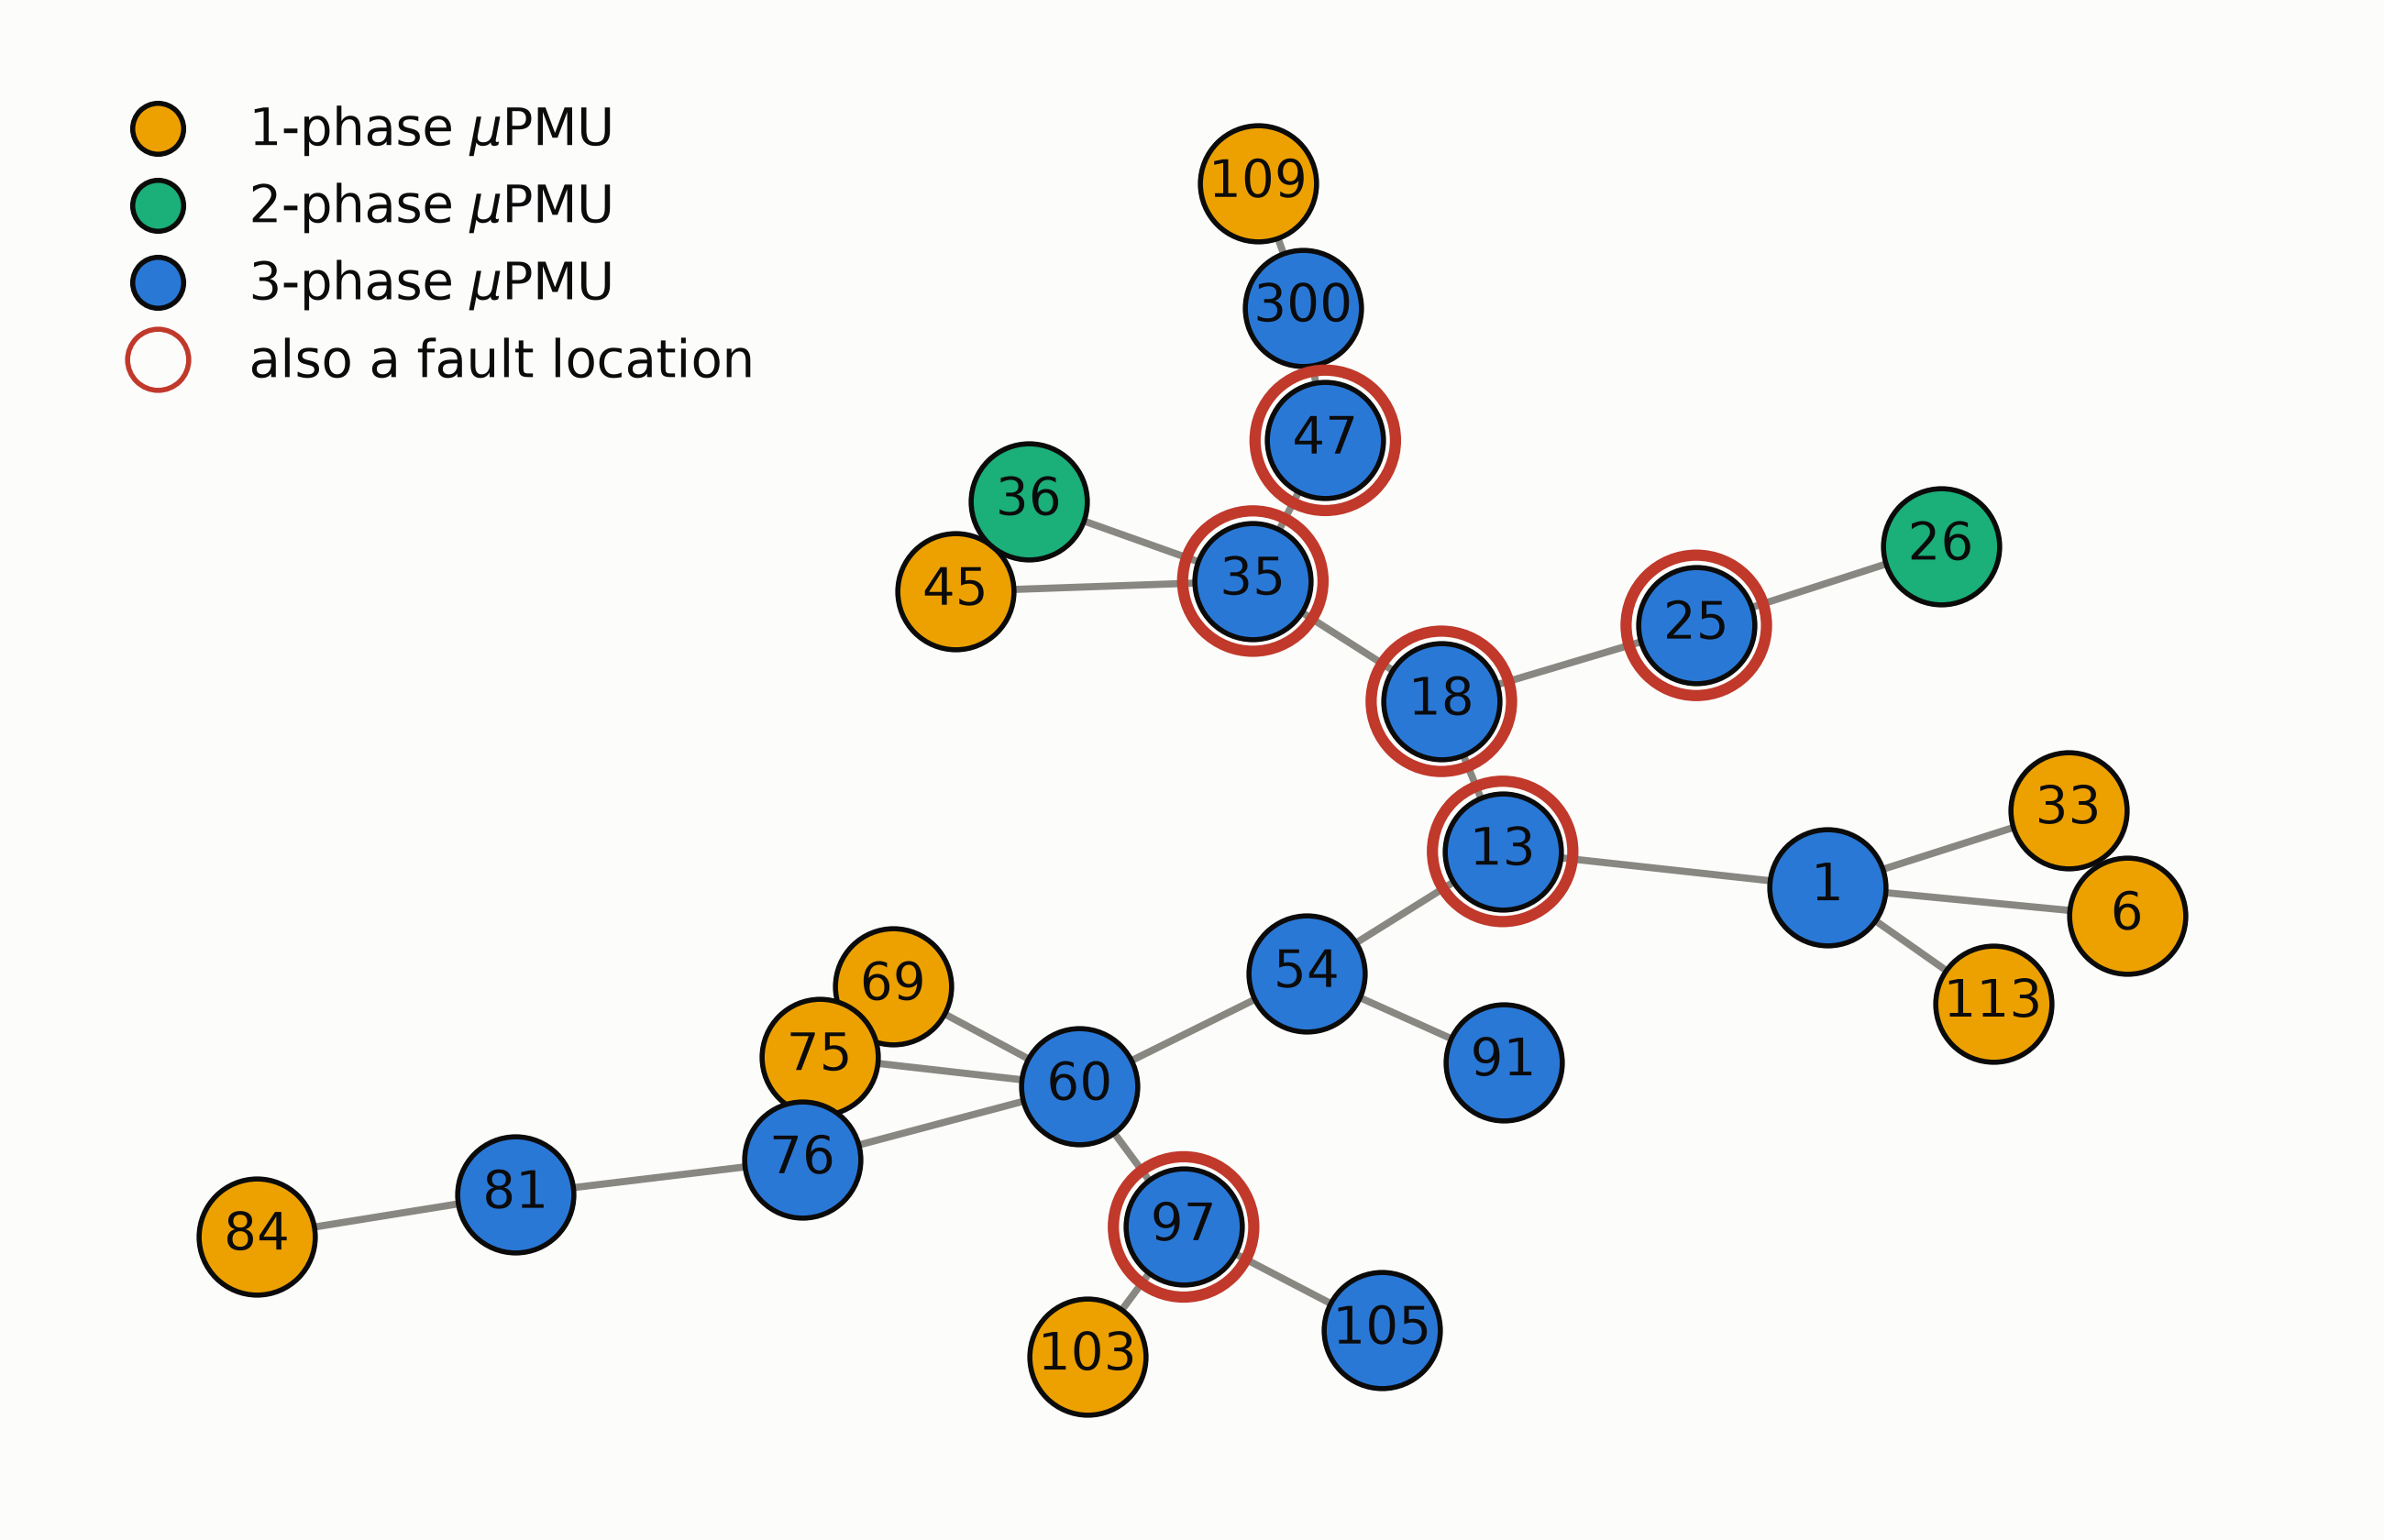
\includegraphics[width=0.7\linewidth]{figures/measured_only_graph.png}
\caption{The measured-only graph of 25 $\mu$PMU buses (colored by phase count) and
24 topology-derived edges, with red rings on the 6 buses that are also fault locations.}
\label{fig:graph}
\end{figure}

Two encoding choices behind Table~\ref{tab:dataset} carry methodological weight. First, the availability mask defines what ``missing'' means throughout this paper: $m_p=1$ marks an available measurement and $m_p=0$ a missing phase or a dropped sensor, so a $\mu$PMU that fails is encoded exactly like one that was never installed. Second, the 70/15/15 partition is taken at the \emph{event} level, so the 40 sliding windows of one event never span more than one split and no window of a test event is seen during training. Voltage channels are z-score normalized using training-split statistics only. We adopt the base paper's dataset-generation methodology but build our own corpus (Section~\ref{sec:repro}); since every model is trained and evaluated on it with identical splits, the comparisons remain fair. Fault severity varies sharply with fault resistance (Fig.~\ref{fig:sig}): for a three-phase-to-ground fault at bus 101, the deepest-sagging $\mu$PMU channel drops $0.83$\,p.u. below its pre-fault level at $0.1\,\Omega$, $0.22$\,p.u. at $1\,\Omega$, and only $0.01$\,p.u. at $10\,\Omega$, which is why high-impedance faults are the hardest class to localize throughout this study.

\begin{figure}[!t]
\centering
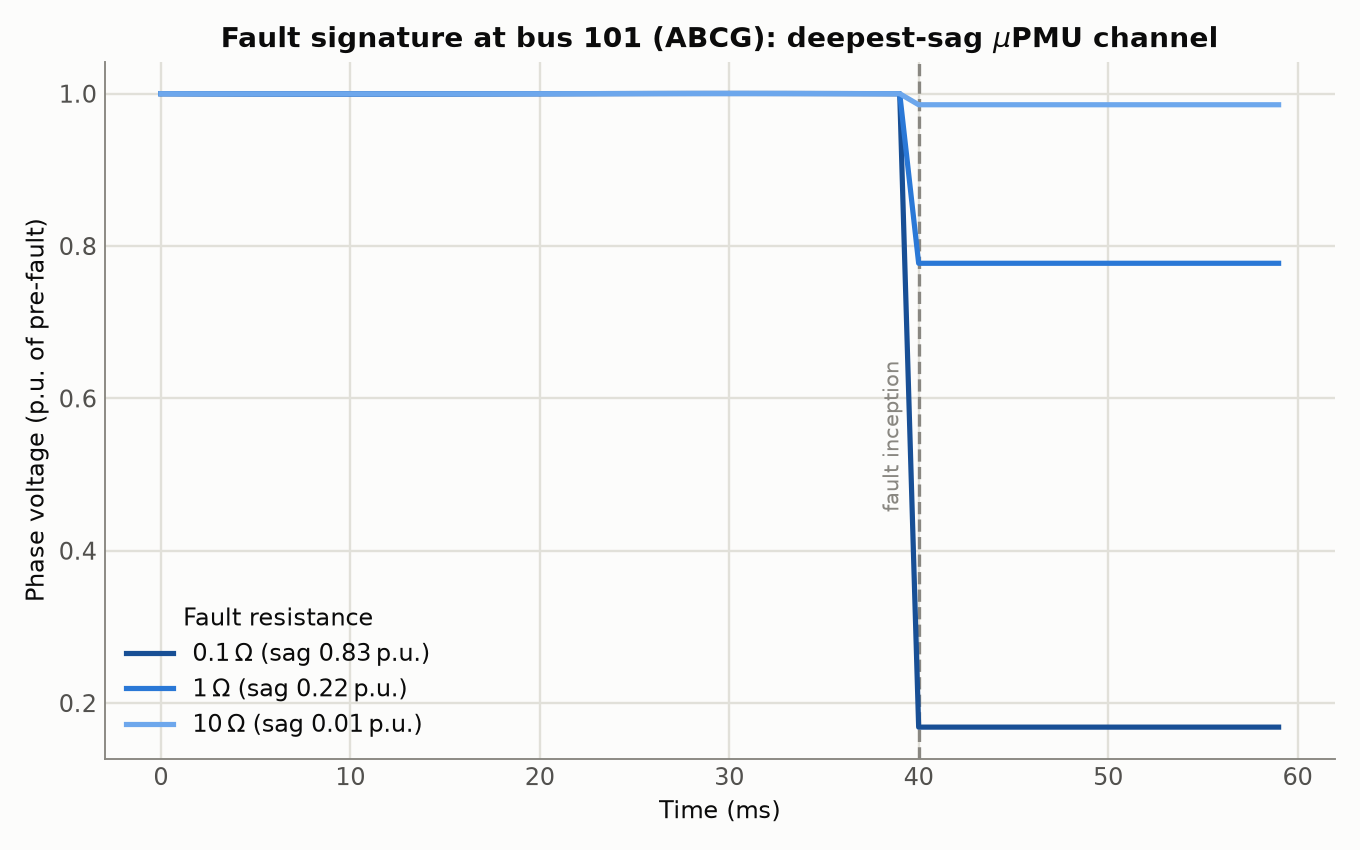
\includegraphics[width=0.7\linewidth]{figures/fault_signature.png}
\caption{Deepest-sagging $\mu$PMU channel for a three-phase-to-ground fault at bus 101,
normalized to its pre-fault mean, showing that sag depth shrinks as fault resistance rises.}
\label{fig:sig}
\end{figure}

% ---------------------------------------------------------------------------
% Dataset configuration + window-level split counts.
%   Frozen corpus: dataset_fullscale_50 (50 runs/scenario)
%   Split counts: paper/tables/dataset_info.tex (scripts/build_dataset_assets.py)
% ---------------------------------------------------------------------------
\begin{table}[!ht]
  \centering
  \caption{Dataset configuration and event-level 70/15/15 split of the 50-run corpus.}
  \label{tab:dataset}
  \footnotesize
  \begin{tabular}{@{}ll@{}}
    \toprule
    \multicolumn{2}{@{}l}{\textit{Simulation configuration}} \\
    \midrule
    Test feeder / simulator   & IEEE 123-bus, 4.16\,kV, 60\,Hz; OpenDSS (OpenDSSDirect.py), Daily mode, 1\,ms step \\
    Fault buses / $\mu$PMUs   & 25 / 25 (single-, two-, and three-phase units) \\
    Fault types / resistances & 11 (3 LG, 3 LL, 3 LLG, 2 three-phase) / 3 (0.1, 1, 10\,$\Omega$) \\
    Load multiplier           & $\mathcal{U}(0.5,\,1.3)$ per run \\
    Scenarios $\times$ runs   & $25 \times 11 \times 3 = 825$ scenarios $\times$ 50 runs \\
    Record / windowing        & 60\,ms record (40\,ms pre-fault); 20-step (20\,ms) windows, 40 per event \\
    Node features $F$ / classes & 6 ($[V_1,V_2,V_3]$ $+$ availability mask $[m_1,m_2,m_3]$) / 26 (25 locations $+$ no-fault) \\
    \addlinespace
    \multicolumn{2}{@{}l}{\textit{Window-level distribution (event-level split)}} \\
    \midrule
    Split      & Fault / No-fault / Total windows (events) \\
    \midrule
    Train      & 577,500 / 577,500 / 1,155,000 (28,875) \\
    Validation & 124,000 / 124,000 / 248,000 (6,200) \\
    Test       & 123,500 / 123,500 / 247,000 (6,175) \\
    Total      & 825,000 / 825,000 / 1,650,000 (41,250) \\
    \bottomrule
  \end{tabular}
\end{table}





\subsection{Baseline Architectures: GRU, RGCN, RGSAGE, RGATv2}

We evaluate the four STGNN architectures of \cite{Karabulut2026} (RGCN, RGSAGE-Mean, RGSAGE-Max, and RGATv2) together with the temporal-only GRU that serves as their non-spatial reference; the GRU has no message-passing stage and is therefore not itself a spatio-temporal GNN. All five follow the designs of \cite{Karabulut2026} unchanged, the one exception being spatial depth, a configuration choice discussed below. On top of the strongest baseline, RGSAGE-Max, this work adds a training method, \emph{dropout-aware training} (Section~\ref{sec:dropout-aware}), and an architecture, \emph{SDR-STGNN}, evaluated as an ablation against it (Section~\ref{sec:sdr}). All five share a common template: a temporal encoder produces one embedding per $\mu$PMU node, an optional spatial stage exchanges information over the measured-only graph, and a shared per-node head with soft voting yields the graph-level prediction. Let $x_v\in\mathbb{R}^{S\times F}$ be the input at $\mu$PMU node $v$ of the $N=25$ node measured-only graph, over the $S=20$ step window with $F=6$ channels, and let $\mathcal N(j)$ denote the neighbors of node $j$ in that graph. A single-layer GRU with 128 hidden units, shared across nodes and applied to each node independently, gives the node embedding of Eq.~\eqref{eq:gru}:

\begin{equation}
\label{eq:gru}
h^{(0)}_v = \mathrm{GRU}(x_v) \in \mathbb{R}^{128},
\qquad v=1,\dots,N .
\end{equation}

The GRU-only baseline stops at Eq.~\eqref{eq:gru} and cannot exploit spatial relationships. The four GNN variants stack $L=4$ message-passing layers (hidden dimension 64, ReLU between layers, self-loops added) over that graph and differ only in the aggregation operator: \emph{RGCN} propagates over the symmetrically normalized adjacency (Eq.~\eqref{eq:rgcn}); \emph{RGSAGE-Mean} and \emph{RGSAGE-Max} concatenate a node's own embedding with a mean- or max-pooled neighborhood before projecting (Eq.~\eqref{eq:rgsage})~\cite{Hamilton2017}; and \emph{RGATv2} applies $H=4$ head GATv2 attention over each node's in-neighbors (Eq.~\eqref{eq:rgat})~\cite{Brody2022}:

\begin{align}
\label{eq:rgcn}
h^{(l+1)} &= \operatorname{ReLU}\!\left(
\tilde D^{-1/2}\tilde A\tilde D^{-1/2}\, h^{(l)} W^{(l)} \right), \\
\label{eq:rgsage}
h^{(l+1)}_j &= \operatorname{ReLU}\!\left( W^{(l)}
\left[ h^{(l)}_j \;\middle\|\;
\rho\big(\{\, h^{(l)}_i : i\in\mathcal N(j) \,\}\big) \right] \right), \\
\label{eq:rgat}
h^{(l+1)}_j &= \operatorname{ReLU}\!\left(
\Big\|_{c=1}^{H} \sum_{i\in\mathcal N(j)\cup\{j\}}
\alpha^{(l,c)}_{ji}\, W^{(l,c)} h^{(l)}_i \right),
\end{align}

where $\tilde A = A+I$ is the adjacency with self-loops and $\tilde D$ its degree matrix, $W^{(l)}$ are the layer weights, $\|$ is concatenation, $\rho$ is mean or max pooling, and $\alpha^{(l,c)}_{ji}$ is the GATv2 attention coefficient of head $c$. These operators are adopted unchanged from \cite{Karabulut2026}.

\textbf{Spatial depth (configuration choice):} The base paper does not state how many message-passing layers its GNN variants use, so the depth had to be selected here. A single hop gave substantially weaker localization, because most fault locations lie more than one hop from any $\mu$PMU (only 6 of 25 fault buses are instrumented); we therefore stack \emph{four} message-passing layers in every GNN variant, fixed for all experiments (Section~\ref{sec:results}).

\textbf{Classification and aggregation:} A shared head (batch normalization, ReLU, dropout $p=0.35$, linear projection to 26 classes) maps the final embedding of every node to logits $z_v$. At inference the per-node class probabilities are summed over all $N$ nodes and the arg-max is the graph-level prediction (soft voting, Eq.~\eqref{eq:vote}). Training minimizes the unweighted node-level cross-entropy of Eq.~\eqref{eq:loss}, in which each window's event label $y$ supervises all nodes; class balance is handled by the balanced corpus (Section~\ref{sec:setup}) rather than by loss weighting.

\begin{align}
\label{eq:vote}
\hat y &= \arg\max_{c\in\{0,\dots,25\}}
\sum_{v=1}^{N} \operatorname{softmax}(z_v)_c , \\
\label{eq:loss}
\mathcal L &= \frac{1}{N}\sum_{v=1}^{N} \mathrm{CE}\!\left(z_v,\, y\right).
\end{align}

\subsection{Deviations from the Base Setup}
\label{sec:repro}

Our setup follows \cite{Karabulut2026} (feeder, $\mu$PMU placement, fault taxonomy, windowing, soft-voting evaluation, and an unweighted cross-entropy objective) but differs in four documented respects: a spatial depth of four message-passing hops, which the base paper leaves unspecified; a $1.65$\,M-window corpus against its $2.5$\,M; a longer schedule of 30 epochs with gradient clipping and learning-rate warmup, against its 15 epochs for the GNN models and 11 for the GRU; and omission of the reconfigured (``green'') topology. All comparisons here use our own corpus and splits, so they are internally consistent and should be read against our own $0.85$ reference point rather than the base paper's absolute scale.

\subsection{Sensor-Dropout Evaluation Protocol}
\label{sec:dropout-eval}

We evaluate robustness to $\mu$PMU failures entirely at \emph{inference} time, with all model parameters fixed, which isolates robustness from any training-time mitigation.

\textbf{Missingness model:} To simulate a lost sensor we select $k$ of the 25 $\mu$PMUs and, for every test window, zero all six input channels of each selected node, both the RMS-voltage and the availability-mask channels. Zeroing the mask is essential: a zero voltage can be a valid reading, so the mask is the definitive indicator that a node is unobserved. This matches the encoding of absent sensors in the dataset (Section~\ref{sec:dataset}), making a failed $\mu$PMU indistinguishable from one that was never instrumented.

\textbf{Graph handling:} A dropped node keeps its edges and still participates in message passing, but its temporal encoder receives an all-zero sequence and emits a zero-valued embedding that propagates to neighbors, exactly the non-informative message the availability-gated model (Section~\ref{sec:sdr}) is designed to suppress. All models see the same graph, so differences arise solely from the message-passing mechanism. (An edge-removal policy was implemented but not used, to avoid confounding topology with dropout.)

\textbf{Dropout sweep and metrics:} We sweep $k \in \{0,1,2,5,10\}$ ($0/4/8/20/40\%$ loss), with $k=0$ the full-observability reference. Dropped sensors are sampled uniformly at random per window, driven by fixed seeds reused across all models so that every architecture sees an identical sequence of dropout realizations on the same frozen test split (Table~\ref{tab:dataset}). Each $(\mathrm{model},k)$ point is averaged over $n_{\mathrm{seed}}=3$ mask realizations and, where stated, over training seeds 42/43/44. Performance is the soft-voted macro-F1 over the 26 classes, giving a macro-F1-versus-$k$ \emph{degradation curve}, from which we derive the \emph{retention} $R(k)$ of Eq.~\eqref{eq:ret} and the \emph{normalized area under the retention curve} (AUDC) of Eq.~\eqref{eq:audc}:

\begin{align}
\label{eq:ret}
R(k) &= \frac{\mathrm{F1}(k)}{\mathrm{F1}(0)}, \\
\label{eq:audc}
\mathrm{AUDC} &= \frac{1}{k_{\max}-k_{\min}}\int_{k_{\min}}^{k_{\max}} R(k)\,dk \in[0,1].
\end{align}

Here $k_{\min}=0$ and $k_{\max}=10$ are the extremes of the sweep, and Eq.~\eqref{eq:audc} is computed by trapezoidal integration over $k \in \{0,1,2,5,10\}$; a higher AUDC means slower degradation. Both metrics are relative to a model's own clean score, so they compare how gracefully models degrade, not how accurate they are.


\subsection{Dropout-Aware Training}

\label{sec:dropout-aware}

Dropout-aware training removes the train-test mismatch exposed in Section~\ref{sec:dropout-eval}: the baselines train with all 25 $\mu$PMUs available but are evaluated under partial observability. We apply the evaluation missingness model as training-time augmentation, drawing a dropout level $k\sim\mathrm{Uniform}\{0,1,2,5\}$ per batch and zeroing $k$ randomly chosen nodes before each forward pass (Algorithm~\ref{alg:aware}). Because $k$ varies batch to batch, every epoch mixes full- and partial-observability cases, so no $\mu$PMU is consistently available and the network cannot depend on any individual sensor. The augmentation touches only the input features, not the graph, architecture, or optimizer, so it applies unchanged to all baselines and to SDR-STGNN (Section~\ref{sec:sdr}). Masking graph elements during training is itself a known regularizer (e.g., DropEdge~\cite{Rong2020}); our contribution is not the primitive but framing $\mu$PMU dropout as a train-test mismatch and studying its mitigation.

% ---------------------------------------------------------------------------
% Dropout-aware training. Requires in the preamble:
%   \usepackage{algorithm}
%   \usepackage{algpseudocode}
%   \usepackage{amsmath,amssymb}
% ---------------------------------------------------------------------------
\begin{algorithm}[t]
  \caption{Dropout-aware training; only the per-batch masking of lines~4--5 differs
           from standard training.}
  \label{alg:aware}
  \begin{algorithmic}[1]
    \Require training batches $\mathcal{B}$; dropout levels
             $\mathcal{K} = \{0,1,2,5\}$; epochs $E$; model $f_\theta$
    \Ensure dropout-aware weights $\theta$
    \For{$e = 1$ \textbf{to} $E$}
      \State reseed the batch-masking RNG \Comment{fresh dropout each epoch}
      \For{each mini-batch $(x, y) \in \mathcal{B}$,
           $x \in \mathbb{R}^{B \times N \times S \times 6}$}
        \State $k \gets \mathrm{Uniform}(\mathcal{K})$ \Comment{one level per batch}
        \State for every window $b \le B$, draw $k$ nodes uniformly and zero all six
               channels of $x_b$ at those nodes
        \State $Z \gets f_\theta(x)$; \ $\mathcal{L} \gets$ mean of Eq.~\eqref{eq:loss}
               over the batch \Comment{$Z \in \mathbb{R}^{B \times N \times 26}$}
        \State backpropagate; clip gradient norm to $1.0$; AdamW step
               \Comment{LR warmup over first 3 epochs}
      \EndFor
    \EndFor
  \end{algorithmic}
\end{algorithm}

All other training details are identical to the baseline (Section~\ref{sec:setup}), so any robustness difference is attributable solely to the augmentation, which is applied only during training and adds no parameters or inference-time cost (measured in Section~\ref{sec:res-cost}).

\subsection{SDR-STGNN: Availability-Gated Graph Aggregation}
\label{sec:sdr}

SDR-STGNN (Sensor Dropout-Robust Spatio-Temporal Graph Neural Network) addresses sensor dropout architecturally and is included as an ablation against dropout-aware training. All five baselines receive the availability mask as input channels $[m_1,m_2,m_3]$, yet none of the operators in Eqs.~\eqref{eq:rgcn}--\eqref{eq:rgat} uses that information, so a dropped node keeps contributing its zero-valued embedding as a non-informative message. SDR-STGNN makes the aggregation of the strongest baseline, RGSAGE-Max, \emph{availability-gated}, so dropped sensors send no messages at all.

\textbf{Availability:} For each input window we derive a binary availability indicator for every node from its three availability-mask channels, given by Eq.~\eqref{eq:avail}:

\begin{equation}
a_i = \mathbf{1}\!\left\{\ \max_{s}\ \max_{p\in\{1,2,3\}}\ m_{i,p}(s) > 0 \right\}
\in \{0,1\},
\label{eq:avail}
\end{equation}

where $m_{i,p}(s)$ is the mask value of phase $p$ at node $i$ and step $s$; thus $a_i=1$ iff any mask channel is active at any step in the window. Every node of the measured-only graph carries a $\mu$PMU, so a single- or two-phase unit still yields $a_i=1$; under the protocol of Section~\ref{sec:dropout-eval} the nodes with $a_i=0$ are exactly those whose sensor has been dropped.

\textbf{Gated aggregation:} Eq.~\eqref{eq:gate} replaces the RGSAGE update of Eq.~\eqref{eq:rgsage} at each of the four message-passing layers, writing $h_i$ for $h^{(l)}_i$ and $h'_j$ for $h^{(l+1)}_j$: the max-aggregation is restricted to available source nodes, and the self-representation is gated by the same availability indicator:

\begin{equation}
\label{eq:gate}
h'_j =
\operatorname{ReLU}\!\left(
W \left[ a_j h_j \;\middle\|\; \mathrm{agg}_j \right]
\right),
\qquad
\mathrm{agg}_j = \!\!\max_{\substack{i \in \mathcal{N}(j)\cup\{j\}\\ a_i=1}}\!\! h_i ,
\end{equation}

where $W$ is the layer projection of Eq.~\eqref{eq:rgsage} and $\mathcal N(j)$, $\|$ are as defined there. Nodes with $a_i=0$ send no messages, and $\mathrm{agg}_j=\mathbf{0}$ when the entire closed neighborhood of $j$ is unavailable. The availability indicators are computed once from the input window (Eq.~\eqref{eq:avail}) and reused across all four layers. The gate adds no parameters, and the shared GRU encoder, four-hop depth, classifier head, and soft voting are identical to RGSAGE-Max; when every sensor is available ($a_i=1$ for all $i$), Eq.~\eqref{eq:gate} reduces exactly to the standard RGSAGE-Max update, so the two are identical under full observability ($k=0$). SDR-STGNN is trained with the dropout-aware augmentation of Section~\ref{sec:dropout-aware}, so the gates are exercised throughout training.

\textbf{Scope of the ablation:} On the same RGSAGE-Max backbone we compare three variants: (i) standard training; (ii) dropout-aware training (ungated, mask as input only); and (iii) SDR-STGNN (dropout-aware training plus availability-gated aggregation). Since everything else is identical, the comparison separates the training-time augmentation from the structural gate (Section~\ref{sec:results}).

\subsection{Experimental Setup}
\label{sec:setup}

All models share one training and evaluation configuration, listed in Table~\ref{tab:setup}. Apart from the variable under study (the message-passing architecture or the augmentation of Section~\ref{sec:dropout-aware}), every part of the pipeline is fixed, so any difference is attributable to that variable alone. The points not covered by Table~\ref{tab:setup} are:

\begin{itemize}
  \item \emph{Batching:} an event-chunk sampler keeps all sliding windows of an event together, consistent with the event-level partition of Table~\ref{tab:dataset}.
  \item \emph{Objective:} imbalance is handled by dataset construction rather than loss weighting. The corpus is 50\% no-fault and the $25\times11\times3$ factorial design represents the 25 fault locations uniformly, so inverse-frequency weighting is unnecessary, matching the unweighted objective of \cite{Karabulut2026}.
  \item \emph{Determinism:} parameter initialization, mini-batch ordering, and the dropout-aware masking are all controlled by one integer seed; no early stopping is used beyond best-validation checkpointing.
  \item \emph{Evaluation:} each trained model is frozen and swept over $k$ under the protocol of Section~\ref{sec:dropout-eval}, with identical fixed mask seeds across models.
\end{itemize}

% ---------------------------------------------------------------------------
% Shared experimental configuration. Values from config/experiment_base.yaml
% and the frozen sweep CLI flags (--gnn-layers 4 --epochs 30
% --grad-clip-norm 1.0 --warmup-epochs 3).
% ---------------------------------------------------------------------------
\begin{table}[!ht]
  \centering
  \caption{Training, evaluation, and software configuration shared by all models.}
  \label{tab:setup}
  \footnotesize
  \begin{tabular}{@{}ll@{}}
    \toprule
    \multicolumn{2}{@{}l}{\textit{Model configuration}} \\
    \midrule
    Temporal encoder        & 1-layer GRU, 128 hidden units, shared across nodes \\
    Spatial layers          & 4 message-passing layers, hidden dimension 64 \\
    Classifier head         & BatchNorm $\to$ ReLU $\to$ dropout $0.35$ $\to$ linear (26); attention dropout 0.3 (RGATv2) \\
    Graph-level readout     & Soft voting over the 25 node predictions \\
    \addlinespace
    \multicolumn{2}{@{}l}{\textit{Optimization}} \\
    \midrule
    Optimizer               & AdamW, learning rate $10^{-3}$, weight decay $10^{-4}$; batch size 32, 30 epochs \\
    Schedule / clipping     & Linear LR warmup over first 3 epochs, constant thereafter; global norm 1.0 \\
    Loss / model selection  & Node-level unweighted cross-entropy; best validation graph macro-F1 \\
    \addlinespace
    \multicolumn{2}{@{}l}{\textit{Evaluation and reporting}} \\
    \midrule
    Training seeds          & 42, 43, 44 (mean\,$\pm$\,std reported) \\
    Dropout levels $k$      & 0, 1, 2, 5, 10 of 25 $\mu$PMUs ($0$--$40\%$ loss) \\
    Mask realizations       & 3 per training seed, seeds shared across models \\
    Metrics                 & Soft-voted macro-F1, retention, AUDC \\
    \addlinespace
    \multicolumn{2}{@{}l}{\textit{Hardware and software}} \\
    \midrule
    GPU                     & 1 $\times$ NVIDIA T1000 (8\,GB) \\
    Software stack          & Python 3.12, PyTorch 2.5.1 (CUDA 12.1), PyTorch Geometric 2.8, \\
                            & OpenDSSDirect.py 0.9.4, NumPy 2.5, scikit-learn 1.9 \\
    \bottomrule
  \end{tabular}
\end{table}

\section{Results}
\label{sec:results}

We first establish the baselines under full observability, then quantify how those fixed models degrade as $\mu$PMUs are removed at inference (the paper's primary evaluation), then compare dropout-aware training against the availability-gated SDR-STGNN, and finally test whether the training-time fix generalizes across architectures. Unless otherwise stated, results are computed on the frozen test split of Table~\ref{tab:dataset} and reported as mean\,$\pm$\,standard deviation over training seeds 42, 43, and 44, consistent with Section~\ref{sec:setup}.
 
\subsection{Baseline Accuracy Under Full Observability}
\label{sec:res-baseline}

Table~\ref{tab:baseline} summarizes the five baselines under full observability ($k=0$); the two macro-F1 columns carry $\pm$\,one standard deviation over seeds 42/43/44, while the per-resistance columns are seed means. The four spatio-temporal GNN models consistently outperform the temporal-only GRU: RGSAGE-Max achieves the highest graph-level macro-F1 of $0.846\pm0.007$, followed by RGSAGE-Mean ($0.786\pm0.023$) and RGCN ($0.712\pm0.017$), whereas the GRU attains only $0.286\pm0.009$. That gap shows the importance of spatial message passing here: because only 6 of the 25 fault locations are instrumented, localization usually requires information to propagate from instrumented buses to unmeasured fault locations (Section~\ref{sec:dataset}), and Eq.~\eqref{eq:gru} alone provides no mechanism for that. For every model the graph-level macro-F1 exceeds the node-level macro-F1, so the soft vote of Eq.~\eqref{eq:vote} consistently improves on individual node predictions.

Accuracy decreases monotonically as fault resistance increases, for every model: RGSAGE-Max, for example, drops from 0.949 at $0.1\,\Omega$ to 0.676 at $10\,\Omega$, reflecting the weaker voltage signatures of high-impedance faults (Section~\ref{sec:dataset}). Fault detection, in contrast, is effectively saturated: all models achieve a no-fault recall of at least $0.9999$ and a no-fault precision of at least $0.972$, so the primary challenge is localization rather than detection. Unlike \cite{Karabulut2026}, RGATv2 is the weakest GNN model here ($0.522\pm0.087$) and the highest in variance across seeds; that spread reflects training instability at the adopted four-layer depth, with metrics taken from the best validated checkpoint of each seed without extensive hyperparameter tuning. Stabilizing RGATv2 at that depth is left as future work.

\begin{table*}[!tb]
\centering
\caption{Baseline macro-F1 under full observability, as mean$\pm$std over seeds 42/43/44, with the best value per column in bold.}

\label{tab:baseline}
\footnotesize
\begin{tabular}{@{}lccccc@{}}
\toprule
\multirow{2}{*}{Model} &
\multicolumn{1}{c}{Graph-level} &
\multicolumn{1}{c}{Node-level} &
\multicolumn{3}{c}{Macro-F1 by fault resistance} \\
\cmidrule(lr){2-2}
\cmidrule(lr){3-3}
\cmidrule(l){4-6}
&
Macro-F1 &
Macro-F1 &
$0.1\,\Omega$ &
$1\,\Omega$ &
$10\,\Omega$ \\
\midrule
RGSAGE-Max
& $\mathbf{0.846 \pm 0.007}$
& $\mathbf{0.718 \pm 0.008}$
& $\mathbf{0.949}$
& $\mathbf{0.893}$
& $\mathbf{0.676}$ \\

RGSAGE-Mean
& $0.786 \pm 0.023$
& $0.660 \pm 0.025$
& $0.906$
& $0.843$
& $0.587$ \\

RGCN
& $0.712 \pm 0.017$
& $0.601 \pm 0.019$
& $0.874$
& $0.792$
& $0.428$ \\

RGATv2
& $0.522 \pm 0.087$
& $0.460 \pm 0.080$
& $0.630$
& $0.574$
& $0.312$ \\

GRU
& $0.286 \pm 0.009$
& $0.150 \pm 0.003$
& $0.410$
& $0.292$
& $0.105$ \\
\bottomrule
\end{tabular}
\end{table*}

These results also justify the spatial depth of four: a single-seed diagnostic depth sweep on RGSAGE-Max rises monotonically from $0.509$ (1 hop) to $0.806$ (4 hops, reduced budget), with the full 30-epoch recipe reaching $0.846$ and no sign of over-smoothing. Because only 6 of the 25 fault buses are instrumented, a single hop cannot reach faults two or more hops from any $\mu$PMU, so the enlarged receptive field is the primary driver of accuracy.

\subsection{Accuracy Degradation Under Sensor Dropout}
\label{sec:res-degrade}

We now freeze each baseline and evaluate it under the dropout sweep of Section~\ref{sec:dropout-eval}. Table~\ref{tab:degradation} summarizes the degradation curves through AUDC (Eq.~\eqref{eq:audc}) and retention at the most severe level ($k=10$, $40\%$ sensor loss); Fig.~\ref{fig:degradation} shows the full curves. Every model declines as sensors are removed, and no baseline retains more than a third of its full-observability macro-F1 at $k=10$.

The results reveal a clear trade-off between clean accuracy and robustness; the training-seed standard deviation stays below $0.06$ at every $k$ for four of the five models and reaches $0.09$ for RGATv2. RGSAGE-Max, the strongest model under full observability, is the least robust, retaining only $5.7\%$ of its clean macro-F1 at $k=10$, while the remaining models retain a larger fraction of their (lower) baseline accuracy. This inversion is not an artifact of normalizing by each model's own clean score: the curves cross in \emph{absolute} macro-F1 as well, RGSAGE-Max falling to $0.048$ at $k=10$ against RGCN's $0.164$ and RGATv2's $0.157$. RGATv2's nominal top-robustness position, by contrast, is indicative only: it has the lowest clean accuracy of the GNNs, the largest seed variance ($\pm0.087$ at $k=0$), and a retention spread of $\pm16.4$ percentage points that overlaps RGCN's, so we do not read it as robustness leadership. The headline inversion does not rest on it either: excluding RGATv2 entirely, RGSAGE-Max still retains $5.7\%$ against RGCN's $23.2\%$. The robust conclusion is that clean accuracy does not predict robustness to sensor loss, since the most accurate model degrades the fastest. This is consistent with the aggregation operators, max-aggregation being the most exposed to the zeroed embedding a dropped node propagates, whereas mean and normalized-sum dilute it (Section~\ref{sec:discussion}), and it motivates the two mitigations of Sections~\ref{sec:dropout-aware} and~\ref{sec:sdr}.


% ---------------------------------------------------------------------------
% Baseline degradation.
%   F1 means from results/dropout_study/degradation_curves.csv
%   AUDC / retention = normalized trapezoid of F1(k)/F1(0) over k in {0,1,2,5,10}
% ---------------------------------------------------------------------------
\begin{table*}[!tb]
  \centering
  \caption{Degradation under sensor dropout for standard (Std) and dropout-aware (DA)
           training, averaged over seeds 42/43/44 with three mask realizations each.
           AUDC and Ret.@10 are computed per seed and then averaged; $\pm$ is one standard
           deviation over training seeds. Bold marks the best \emph{absolute} macro-F1 per
           column. The relative columns are deliberately left unbolded: they normalize by
           each model's own clean score, so a low-accuracy model can lead without being
           preferable, and under standard training their seed spread overlaps across
           models (Section~\ref{sec:res-degrade}).}
  \label{tab:degradation}
  \scriptsize
  \setlength{\tabcolsep}{3pt}
  \begin{tabular}{@{}lccccccccccc@{}}
    \toprule
    \multirow{2}{*}{Model}
      & \multicolumn{5}{c}{Standard-training macro-F1 at $k$}
      & \multicolumn{2}{c}{DA macro-F1}
      & \multicolumn{2}{c}{AUDC} & \multicolumn{2}{c}{Ret.@10 (\%)} \\
    \cmidrule(lr){2-6}\cmidrule(lr){7-8}\cmidrule(lr){9-10}\cmidrule(l){11-12}
      & $k{=}0$ & $k{=}1$ & $k{=}2$ & $k{=}5$ & $k{=}10$
      & $k{=}0$ & $k{=}10$
      & Std & DA & Std & DA \\
    \midrule
    RGATv2      & 0.522 & 0.490 & 0.444 & 0.302 & 0.157 & 0.553 & 0.505
                & $0.626{\pm}0.112$ & $0.961{\pm}0.014$ & $31.0{\pm}16.4$ & $91.4{\pm}2.8$ \\
    RGCN        & 0.712 & 0.664 & 0.610 & \textbf{0.418} & \textbf{0.164} & 0.613 & 0.533
                & $0.608{\pm}0.047$ & $0.940{\pm}0.011$ & $23.2{\pm}\phantom{0}7.0$ & $87.0{\pm}1.9$ \\
    RGSAGE-Mean & 0.786 & 0.720 & \textbf{0.647} & 0.393 & 0.108 & 0.673 & 0.550
                & $0.541{\pm}0.041$ & $0.922{\pm}0.034$ & $13.8{\pm}\phantom{0}6.4$ & $81.9{\pm}8.4$ \\
    GRU         & 0.286 & 0.273 & 0.252 & 0.111 & 0.051 & 0.300 & 0.078
                & $0.522{\pm}0.081$ & $0.781{\pm}0.038$ & $17.9{\pm}\phantom{0}4.4$ & $25.4{\pm}5.8$ \\
    RGSAGE-Max  & \textbf{0.846} & \textbf{0.736} & 0.590 & 0.236 & 0.048 & \textbf{0.839} & \textbf{0.674}
                & $0.402{\pm}0.020$ & $0.913{\pm}0.006$ & $\phantom{0}5.7{\pm}\phantom{0}1.8$ & $80.3{\pm}1.3$ \\
    \bottomrule
  \end{tabular}
\end{table*}

% ---------------------------------------------------------------------------
% Degradation curves for all baselines + SDR-STGNN.
%   figures/sdr_degradation_all.png
% ---------------------------------------------------------------------------
\begin{figure}[!ht]
  \centering
  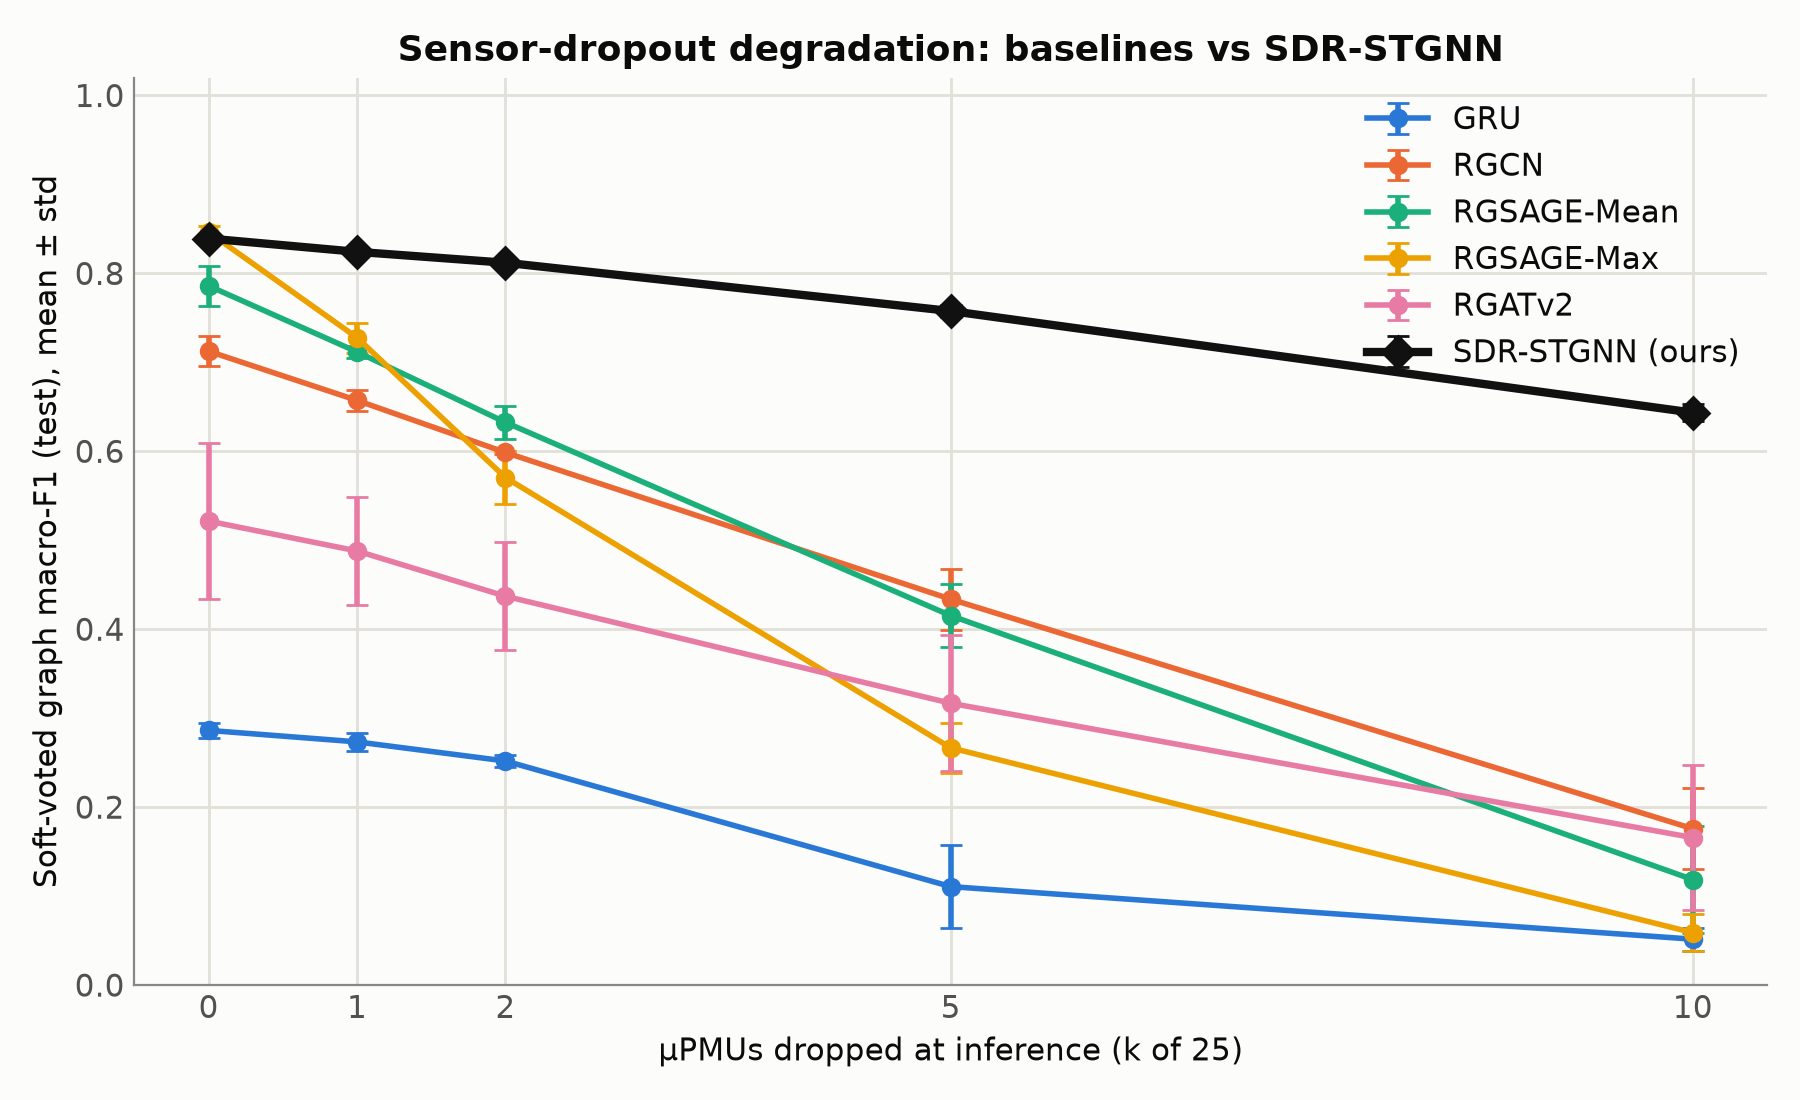
\includegraphics[width=0.7\linewidth]{figures/sdr_degradation_all.png}
  \caption{Soft-voted macro-F1 against the number $k$ of dropped $\mu$PMUs for the five
           baselines and SDR-STGNN (black), with error bars of $\pm1$ std over seeds 42/43/44.}
  \label{fig:degradation}
\end{figure}


\subsection{Effect of Dropout-Aware Training}
\label{sec:res-aware}

Table~\ref{tab:aware} compares four ways to cope with sensor loss on the identical sweep, all on the RGSAGE-Max backbone: standard training (dropped nodes zeroed), an impute-then-infer baseline, dropout-aware training, and the availability-gated SDR-STGNN; the SDR-STGNN curve is also plotted in Fig.~\ref{fig:degradation}.

\textbf{Imputation baseline:} A natural alternative to a training-time fix is to reconstruct dropped sensors before inference. As a lightweight control, the no-training analogue of graph-based imputation~\cite{zhang2025}, we fill each dropped node's three voltage channels with the per-timestep mean of its \emph{available} undirected $1$-hop neighbors and present the result to the standard-trained model as observed (mask set to $1$, the most favorable setting for imputation); dropped nodes are selected exactly as in the zeroing sweep, so the only change is the fill. Imputation gains little over zeroing (AUDC $0.402\!\to\!0.476$; $k=10$ retention $5.7\%\!\to\!11.8\%$) and stays far below dropout-aware training (AUDC $0.913$), because the reconstructed values are still fed to a model never trained to distrust them.

Dropout-aware training raises the AUDC of RGSAGE-Max from $0.402$ to $0.913$ and its $k=10$ retention from $5.7\%$ to $80.3\%$: where the standard model collapses to a macro-F1 of $0.048$ at $40\%$ sensor loss, the dropout-aware variant still reaches $0.674\pm0.017$, an absolute gain of $0.626$ macro-F1 points. Clean performance is essentially unchanged ($0.839\pm0.011$ against $0.846\pm0.007$ at $k=0$, within one standard deviation and not significant at $p=0.181$; Section~\ref{sec:res-significance}), and because the augmentation alters only the training data it adds no parameters and no measurable inference-time cost, both confirmed by measurement in Section~\ref{sec:res-cost}.

The availability-gated SDR-STGNN matches that robustness but does not exceed it: its AUDC is $0.892$ and its $k=10$ retention $75.2\%$, both slightly below the ungated model, and its curve lies below the dropout-aware curve for all $k\ge1$. At $k=0$ the gate of Eq.~\eqref{eq:gate} is inactive, so the architecture reduces exactly to its backbone and the two dropout-aware variants score identically ($0.839$, within seed noise). The structural gate thus adds nothing beyond the training-time augmentation, leaving dropout-aware training the most effective and most practical mitigation evaluated here.

% ---------------------------------------------------------------------------
% Dropout-aware comparison.
%   standard / aware = results/dropout_study{,_aware}/degradation_curves.csv
%                      (RGSAGE-Max, seeds 42/43/44)
%   sdr              = results/dropout_study_sdr/degradation_curves.csv
%                      (SDR-STGNN, seeds 42/43/44)
% ---------------------------------------------------------------------------
\begin{table*}[!tb]
  \centering
  \caption{Test-time and training-time mitigations on the RGSAGE-Max backbone, as
           mean\,$\pm$\,std over seeds 42/43/44, with the best value per column in bold.
           The sweep covers the same $k$ grid as Table~\ref{tab:degradation}; AUDC and
           Ret.@10 are computed per seed and then averaged, so they may differ in the last
           digit from ratios recomputed from the three-decimal entries shown. All four
           variants share one backbone and one clean score, so the relative columns are
           directly comparable here, unlike those of Table~\ref{tab:degradation}.}
  \label{tab:aware}
  \footnotesize
  \setlength{\tabcolsep}{4pt}
  \begin{tabular}{@{}lccccccc@{}}
    \toprule
    Variant & $k{=}0$ & $k{=}1$ & $k{=}2$ & $k{=}5$ & $k{=}10$ & AUDC & Ret.@10 (\%) \\
    \midrule
    Standard training (zeroing)
      & $\mathbf{0.846}{\pm}\mathbf{0.007}$
      & $0.736{\pm}0.013$
      & $0.590{\pm}0.024$
      & $0.236{\pm}0.023$
      & $0.048{\pm}0.015$
      & $0.402{\pm}0.020$ & $5.7{\pm}1.8$ \\
    Mean-imputation (standard)
      & $0.846{\pm}0.006$
      & $0.739{\pm}0.014$
      & $0.637{\pm}0.023$
      & $0.336{\pm}0.035$
      & $0.099{\pm}0.027$
      & $0.476{\pm}0.034$ & $11.8{\pm}3.3$ \\
    Dropout-aware training
      & $0.839{\pm}0.011$
      & $\mathbf{0.827}{\pm}\mathbf{0.011}$
      & $\mathbf{0.815}{\pm}\mathbf{0.011}$
      & $\mathbf{0.774}{\pm}\mathbf{0.013}$
      & $\mathbf{0.674}{\pm}\mathbf{0.017}$
      & $\mathbf{0.913}{\pm}\mathbf{0.006}$ & $\mathbf{80.3}{\pm}\mathbf{1.3}$ \\
    SDR-STGNN (gated)
      & $0.839{\pm}0.002$
      & $0.827{\pm}0.003$
      & $0.813{\pm}0.004$
      & $0.758{\pm}0.006$
      & $0.631{\pm}0.010$
      & $0.892{\pm}0.007$ & $75.2{\pm}1.3$ \\
    \bottomrule
  \end{tabular}
\end{table*}


\subsection{Dropout-Aware Training Across Architectures}
\label{sec:res-agnostic}

To test whether the gain is specific to the RGSAGE-Max backbone, we retrain every baseline with the identical augmentation and re-evaluate under the same sweep; the resulting values appear in the dropout-aware columns of Table~\ref{tab:degradation}. Robustness improves for all five architectures. The four spatial GNNs rise from AUDC $0.40$--$0.63$ to $0.91$--$0.96$ and from at most $31\%$ to $80$--$91\%$ retention at $k=10$. The cost in clean accuracy, however, is not uniform: RGSAGE-Max loses under $0.01$ macro-F1 at $k=0$, but RGCN drops $0.099$ ($0.712\to0.613$) and RGSAGE-Mean $0.113$ ($0.786\to0.673$), so the result that robustness comes at no cost to clean accuracy holds for the backbone we adopt rather than for the family as a whole. We did not isolate the cause; one untested explanation is that max-pooling selects a single surviving neighbor activation and is therefore largely unperturbed by masking, whereas mean and normalized-sum aggregation have the statistics of their neighborhood averages shifted by it, making the clean objective harder to fit within the same training budget. Because retention normalizes by each model's own clean score, the relative leaders are again not the strongest in absolute terms: dropout-aware RGSAGE-Max reaches $0.674$ macro-F1 at $k=10$, well above RGATv2's $0.505$ despite RGATv2's higher retention. The GNN-free GRU also improves (AUDC $0.52\to0.78$) but its retention stays limited ($25\%$), since without a spatial mechanism it cannot exploit surviving sensors. Robustness recovery is therefore a general property of the training scheme, strongest where the architecture can route information around a failure.

\subsection{Statistical Significance}
\label{sec:res-significance}

Every comparison above is a mean over three training seeds, which is a small sample, so we state explicitly which differences survive a test. Table~\ref{tab:significance} reports paired two-sided $t$-tests on the seed-wise differences ($n=3$, $\mathrm{df}=2$) for the six mitigation claims, Holm--Bonferroni adjusted across the family with the two expected null results included rather than exempted. The seed is the paired unit because every variant is trained from the same three seeds on identical data and splits, so the pairing removes seed-to-seed variation in training difficulty as a nuisance factor. We deliberately do not rely on a Wilcoxon signed-rank test: at $n=3$ its smallest attainable two-sided $p$-value is $0.25$, so it cannot reject at any conventional level whatever the effect size, and reporting it would only obscure that this is a property of the sample size rather than of the data.

The positive claims survive adjustment. Dropout-aware training gains $0.626$ macro-F1 at $k=10$ (95\% CI $[0.557, 0.695]$, $p_{\text{Holm}}=0.003$), $74.6$ percentage points of retention and $0.511$ AUDC over standard training (both $p_{\text{Holm}}=0.003$), and exceeds mean-imputation by $0.574$ macro-F1 at $k=10$ ($p_{\text{Holm}}=0.008$). Extending the same test to every level and every architecture, the gain is significant at each $k\ge1$ ($p_{\text{Holm}}\le0.042$) and the AUDC gain is significant for all five architectures ($p_{\text{Holm}}\le0.027$), so the cross-architecture claim of Section~\ref{sec:res-agnostic} does not rest on the backbone alone. The two claims we make \emph{as} null results test as null: the clean-accuracy change at $k=0$ is $-0.008$ with a CI spanning zero ($p=0.181$), and dropout-aware training's $0.021$ AUDC edge over SDR-STGNN is not significant ($p=0.098$), which is the statistical form of ``matches but does not surpass''. Mean-imputation's $0.051$ gain over zeroing at $k=10$ is likewise not significant ($p=0.102$), sharpening Section~\ref{sec:res-aware}: on this evidence imputation is not distinguishable from doing nothing.

Two cross-architecture orderings need an explicit caveat, which reflects the limit of a three-seed design rather than a weakness in the effects themselves. The clean-accuracy ranking of Table~\ref{tab:baseline} reaches only $p=0.023$ for its top pair (RGSAGE-Max over RGSAGE-Mean) and no adjacent pair survives Holm adjustment across the four. Neither does the accuracy--robustness inversion: RGCN's absolute macro-F1 at $k=10$ exceeds RGSAGE-Max's in every one of the three seeds, by a factor of $2.4$ to $6.7$ ($\Delta=0.116$), yet $p=0.076$, because the \emph{size} of the gap varies with the seed even though its sign does not. A complementary bootstrap locates that noise. Resampling the $6{,}175$ test events at $k=0$ --- events, not windows, since one simulated fault contributes $40$ correlated windows --- puts the RGSAGE-Max-over-RGSAGE-Mean gap at $+0.042$ macro-F1 with a 95\% CI of $[+0.034, +0.051]$ ($p<0.001$) for a single seed, and the standard-versus-dropout-aware clean gap at $-0.001$, CI $[-0.008, +0.005]$. Test-set sampling error is several times narrower than the corresponding seed-level interval, so what bounds the architecture-ranking conclusions is the number of training seeds, not the size of the test set, and we report those orderings as consistent observations at three seeds rather than as significant differences.

% ---------------------------------------------------------------------------
% Significance tests.  Generated by scripts/run_significance_tests.py from the
% per-seed values already on disk (results/dropout_study{,_aware,_sdr}/
% degradation_curves.csv + results/dropout_study_impute/imputation_summary.json).
% Verbatim copy of paper/tables/significance.tex -- regenerate, do not hand-edit.
% ---------------------------------------------------------------------------
\begin{table}[!tb]
  \centering
  \caption{Paired two-sided $t$-tests over training seeds 42/43/44
           ($n=3$, $\mathrm{df}=2$) on the mitigation claims, all on the
           RGSAGE-Max backbone. $\Delta$ is the mean seed-wise difference in
           the stated metric (F1 points, AUDC, or percentage points for
           Ret.@10); $p_{\text{Holm}}$ is Holm-Bonferroni adjusted over all
           six tests, the two expected null results included. Std\ =\ standard
           training, DA\ =\ dropout-aware.}
  \label{tab:significance}
  \scriptsize
  \setlength{\tabcolsep}{3pt}
  \begin{tabular}{@{}lcccc@{}}
    \toprule
    Comparison & $\Delta$ & $95\%$ CI & $p$ & $p_{\text{Holm}}$ \\
    \midrule
    DA vs.\ Std, clean F1 ($k{=}0$) & $-0.008$ & $[-0.024,\,+0.009]$ & $0.181$ & $0.196$ \\
    DA vs.\ Std, F1 at $k{=}10$ & $+0.626$ & $[+0.557,\,+0.695]$ & $<\!0.001$ & $0.003$ \\
    DA vs.\ Std, Ret.@10 & $+74.6$ & $[+67.2,\,+82.0]$ & $<\!0.001$ & $0.003$ \\
    DA vs.\ Std, AUDC & $+0.511$ & $[+0.450,\,+0.571]$ & $<\!0.001$ & $0.003$ \\
    DA vs.\ imputation, F1 at $k{=}10$ & $+0.574$ & $[+0.449,\,+0.699]$ & $0.003$ & $0.008$ \\
    DA vs.\ SDR-STGNN, AUDC & $+0.021$ & $[-0.010,\,+0.052]$ & $0.098$ & $0.196$ \\
    \bottomrule
  \end{tabular}
\end{table}

\subsection{Computational Cost}
\label{sec:res-cost}

Table~\ref{tab:runtime} measures the cost claims made above. Dropout-aware training alters only the training data, so it must leave inference untouched, and it does: the standard and dropout-aware RGSAGE-Max checkpoints have identical parameter counts ($95{,}258$) and time identically, $0.639$ against $0.640$\,ms per single-event forward pass --- a $0.3\%$ difference, an order of magnitude inside the $\pm0.02$\,ms run-to-run spread --- at $6{,}038$ windows/s in both cases. The augmentation's cost falls entirely on training and is small: $13.7$ against $13.4$ minutes per epoch, a $2.7\%$ overhead for drawing and applying the masks, or $0.2$\,h over a $6.9$\,h run.

SDR-STGNN's gate, by contrast, is a genuine inference cost. It adds no parameters, being a multiplicative mask rather than a learned module, but it raises single-event latency by $18\%$ ($0.755$ against $0.639$\,ms) and lowers throughput by $2\%$, because availability has to be recomputed and applied at every hop. Read with Section~\ref{sec:res-aware}, where it does not exceed the augmentation, the gate buys no measured robustness for that latency.

The remaining columns supply implementation details. Activation memory is $145$\,MiB at batch $32$ for every model, because all five share the same GRU-128 temporal encoder (Section~\ref{sec:setup}), whose per-node sequence activations dominate the graph layers; the weights themselves span only $0.21$--$1.40$\,MiB, so model size is not the binding constraint for a substation deployment. Training one seed took $4.7$\,h (GRU) to $12.3$\,h (RGATv2, $24.6$ minutes per epoch for its four attention heads). Convergence is the one number that is not comfortable: the best validation epoch averages $27.7$--$28.7$ of the $30$-epoch budget for the three stable spatial GNNs, so they were still improving when training stopped and the accuracies reported here should be read as a floor rather than a converged optimum. Only the temporal-only GRU ($25.0$) and RGATv2 ($24.7$) peak appreciably earlier, and for RGATv2 that reflects its instability at this depth rather than convergence: its best epoch ranges from $19$ to $29$ across the three seeds.

% ---------------------------------------------------------------------------
% Runtime / efficiency.  Generated by scripts/run_runtime_benchmark.py:
%   inference columns measured on this machine's T1000 over synthetic batches;
%   training columns read from each run's metrics_by_epoch.csv (train_seconds,
%   argmax of val_graph_f1).  Verbatim copy of paper/tables/runtime.tex.
% ---------------------------------------------------------------------------
\begin{table*}[!tb]
  \centering
  \caption{Cost of each model and of the dropout-aware augmentation, on one
           NVIDIA T1000 (8\,GB). Inference is timed over synthetic batches of
           the true input shape $[B,25,20,6]$: single-event latency at $B{=}1$
           and throughput at $B{=}32$, with the activation memory the
           forward pass allocates (peak minus resident weights and cuBLAS
           workspace). Training columns are wall-clock numbers recorded by the
           runs that produced the results (30 epochs, mean over seeds
           42/43/44); ``best ep.'' is the epoch of highest validation
           soft-voted graph F1, i.e.\ the checkpoint actually reported.
           Std\ =\ standard training, DA\ =\ dropout-aware.}
  \label{tab:runtime}
  \footnotesize
  \setlength{\tabcolsep}{5pt}
  \begin{tabular}{@{}llccccccc@{}}
    \toprule
    \multirow{2}{*}{Model} & \multirow{2}{*}{Train.}
      & \multirow{2}{*}{Params}
      & \multicolumn{3}{c}{Inference} & \multicolumn{3}{c}{Training} \\
    \cmidrule(lr){4-6}\cmidrule(l){7-9}
      & & & Lat. (ms) & Windows/s & Act.\ mem. (MiB)
      & min/epoch & Total (h) & Best ep. \\
    \midrule
    GRU & Std & $55.8$k & $0.35$ & $5{,}548$ & $145$ & $9.4$ & $4.7$ & $25.0$ \\
    RGCN & Std & $74.8$k & $0.69$ & $5{,}934$ & $145$ & $10.6$ & $5.3$ & $27.7$ \\
    RGSAGE-Mean & Std & $95.3$k & $0.90$ & $5{,}606$ & $145$ & $10.8$ & $5.4$ & $28.3$ \\
    RGSAGE-Max & Std & $95.3$k & $0.64$ & $6{,}038$ & $145$ & $13.4$ & $6.7$ & $28.7$ \\
    RGATv2 & Std & $366.4$k & $1.38$ & $4{,}670$ & $145$ & $24.6$ & $12.3$ & $24.7$ \\
    RGSAGE-Max & DA & $95.3$k & $0.64$ & $6{,}038$ & $145$ & $13.7$ & $6.9$ & $28.0$ \\
    SDR-STGNN & DA & $95.3$k & $0.75$ & $5{,}909$ & $145$ & $13.9$ & $7.0$ & $29.0$ \\
    \bottomrule
  \end{tabular}
\end{table*}

\section{Discussion}
\label{sec:discussion}
 
\subsection{Robustness Ranking of the Baseline Architectures}

The five baselines expose an inverse relationship between clean accuracy and robustness: the accuracy ranking (RGSAGE-Max $>$ RGSAGE-Mean $>$ RGCN $>$ RGATv2 $>$ GRU) is essentially reversed by the robustness (AUDC) ranking (Tables~\ref{tab:baseline}--\ref{tab:degradation}). The clearest signal is the inversion at the extremes: the strongest clean model degrades the fastest, retaining only $5.7\%$ at $k=10$ against RGCN's $23.2\%$, in the same direction in all three seeds although the three-seed paired test does not reach significance ($p=0.076$, Section~\ref{sec:res-significance}). The ordering \emph{among} the mid-tier baselines is indicative rather than established, because the spatial depth was selected on RGSAGE-Max and then applied unchanged to every architecture (Section~\ref{sec:res-baseline}); a per-architecture depth could plausibly reorder them, and would in particular raise RGATv2, whose high relative retention rests on a clean score depressed by instability at that depth.

This ordering follows from how each operator treats the zeroed embedding a dropped sensor propagates (Section~\ref{sec:dropout-eval}). The max pooling of Eq.~\eqref{eq:rgsage} forwards the single largest activation in a neighborhood, so one corrupted message can dominate a live node's update, making RGSAGE-Max the most fragile despite being the strongest clean model, whereas the normalized sum of Eq.~\eqref{eq:rgcn} and mean pooling average that message against surviving ones and degrade more gracefully. Attention (Eq.~\eqref{eq:rgat}) could in principle down-weight a dropped neighbor, but its coefficients are computed from features and are not availability-aware. GRU performs no spatial aggregation, so it is insensitive to neighbors' dropout but capped by the absence of spatial reasoning.

The aggregation operator is therefore a weak lever for robustness: even the most robust baseline retains under a third of its accuracy at $40\%$ dropout. Deployment-level robustness comes from training instead. Dropout-aware training raises retention from $5.7\%$ to $80.3\%$ on the RGSAGE-Max backbone (Table~\ref{tab:aware}) and, altering only the input masking, applies unchanged to every architecture (Table~\ref{tab:degradation}, DA columns). SDR-STGNN confirms this from the opposite side: silencing every dropped node at every hop also removes the multi-hop paths that would otherwise route information around a failure, so the gate adds nothing over the augmentation. Practically, on this feeder an operator could lose roughly 10 of 25 $\mu$PMUs to maintenance or communication faults while macro-F1 stays above $0.67$, provided the model is trained with the augmentation, which supports resilient monitoring of distribution feeders (relevant to UN SDG~7 and SDG~11) without additional sensing hardware.

\subsection{Why Dropout-Aware Training Works}
\label{sec:disc-mechanism}

It is worth separating \emph{that} the augmentation works from \emph{why}, because the mechanism determines when it should be expected to transfer. Each node's input carries three availability-mask channels alongside its three phase voltages (Section~\ref{sec:dataset}), and those channels are not trivial: only 14 of the 25 $\mu$PMUs are three-phase, so the rest present patterns such as $(1,0,0)$. They are, however, entirely \emph{static} --- identical in every training window and at every timestep, because the phase instrumentation of a feeder does not change. A network trained on that corpus can therefore read the mask only as a fixed per-node fingerprint, never as a live availability signal, and it never receives a gradient from a node whose availability changes. Dropping a sensor at inference zeroes all six of its channels, so its mask becomes $(0,0,0)$: a pattern that node has never once presented during training. The model has no learned response to it and instead reads the zeroed voltages as a legitimate near-zero measurement --- and the max-aggregation argument above explains why one such reading then dominates a live node's update. Dropout-aware training is the first thing that makes the mask vary within a node's own history, so $(0,0,0)$ acquires the meaning ``this neighbor is dark now'', and the network learns the down-weighting for itself, from data, rather than being handed it by the architecture.

Three of our results are what that account predicts. First, an explicit architectural gate should then be largely redundant, because the model has already learned the function the gate hard-codes --- and SDR-STGNN does not exceed the augmentation ($\Delta$AUDC $=0.021$, $p=0.098$; Table~\ref{tab:significance}). Second, supplying plausible numbers should not substitute for the training signal, because the deficit is misplaced trust rather than absent values: mean-imputation hands the standard-trained model a neighbor-averaged reading and even sets the mask to $1$, yet gains only $0.051$ macro-F1 at $k=10$ ($p=0.102$), while the augmentation gains $0.574$ over it. Third, the augmentation can only exploit redundancy the architecture can actually reach, so its benefit should scale with spatial connectivity --- and the AUDC gain is largest on RGSAGE-Max ($+0.511$) and smallest on the temporal-only GRU ($+0.259$), whose retention at $k=10$ stops at $25\%$ against RGSAGE-Max's $80\%$ precisely because it has no message passing with which to route around a dark node. Taken together: dropout-aware training does not reconstruct the missing measurement, it trains the model out of depending on any particular one, and the four-hop receptive field over a $25$-node tree is what leaves it somewhere else to look.

\subsection{Limitations}

Nine limitations bound these findings. All experiments use the IEEE 123-bus feeder in its default configuration, so generalization across network sizes and topologies, including the reconfigured (``green'') topology of \cite{Karabulut2026}, remains open (Section~\ref{sec:repro}). Our missingness model drops sensors independently and uniformly at random per window, whereas real $\mu$PMU failures are often correlated (co-located units, a shared communication path, or a substation outage fail together) and persistent, so structured failures may degrade, and respond to mitigation, differently. Every number reported here is consequently an average over random sensor subsets rather than a worst case: because only 6 of the 25 fault buses are instrumented, losing the $\mu$PMUs nearest a fault should hurt considerably more than losing the same number at random, and we did not evaluate that targeted setting. Voltages are also taken directly from the simulator, without additive measurement noise, quantization, or communication latency, so the full-observability accuracies are optimistic relative to field $\mu$PMU data. Our $1.65$\,M-window corpus yields a strongest-baseline macro-F1 of $0.846$, not directly comparable to \cite{Karabulut2026}, which uses a different corpus (Section~\ref{sec:repro}). The four message-passing layers were chosen from a single-seed depth sweep on RGSAGE-Max and then held fixed for all five architectures; combined with RGATv2's seed variance ($\pm0.087$ at $k=0$), this makes the cross-architecture orderings in Tables~\ref{tab:baseline} and~\ref{tab:degradation} indicative rather than firm (Section~\ref{sec:res-degrade}). Our imputation comparison covers only lightweight graph mean-imputation (Section~\ref{sec:res-aware}), not learned reconstruction such as the Dirichlet/contrastive pipeline of \cite{zhang2025} or the VGAE of \cite{fan2024}, so whether a stronger imputer could close the gap is unresolved. Statistical power is bounded by the three training seeds: the mitigation effects are large enough to clear Holm adjustment at $n=3$ (Table~\ref{tab:significance}), but the cross-architecture orderings are not, and a nonparametric test cannot reject at this sample size at all, so settling those orderings would need more seeds rather than a different test (Section~\ref{sec:res-significance}). Finally, dropout-aware training samples $k\in\{0,1,2,5\}$, so the $k=10$ evaluation probes beyond the training distribution; recovery remains strong there, but we ran no ablation over the training dropout grid, leaving open whether including $k=10$ during training would raise the $k=10$ result further or cost additional clean accuracy.

\section{Conclusion and Future Work}
\label{sec:conclusion}

Building on the STGNN fault-localization methodology of \cite{Karabulut2026}, this work contributes a measurement and a negative result. The measurement is that clean accuracy is an unreliable indicator of robustness to $\mu$PMU loss: the highest-performing baseline under full observability degraded the fastest as sensors were removed, in absolute as well as relative terms. The negative result is that an availability-gated architecture, SDR-STGNN, achieved comparable but not superior robustness to a purely training-time fix, so on this task the aggregation operator is a weak lever and robustness is better bought during training. That fix, dropout-aware training, raised the retained macro-F1 at $40\%$ sensor dropout from $5.7\%$ to $80.3\%$ on the RGSAGE-Max backbone ($p_{\text{Holm}}=0.003$) at measured parity in inference latency and parameter count and with no measurable loss of clean accuracy, and improved every architecture tested, although on RGCN and RGSAGE-Mean it cost roughly $0.1$ macro-F1 under full observability. Future work will investigate correlated and spatially structured sensor failures, worst-case rather than average-case sensor loss, larger and more diverse feeder datasets, cross-topology generalization to reconfigured feeders, and adaptive availability-gating mechanisms.
 
\section*{Acknowledgements}

The authors thank the Department of Computer Science and Engineering, Amrita School of Computing, Coimbatore, Amrita Vishwa Vidyapeetham, for the institutional support that made this work possible.

% ---------------------------------------------------------------------------
% Elsevier requires this declaration at the end of the manuscript, immediately
% above the references, under exactly this section title. Template wording from
% elsevier.com/about/policies-and-standards/the-use-of-generative-ai-and-ai-
% assisted-technologies-in-writing-for-elsevier (verified 2026-08-13).
% ---------------------------------------------------------------------------
\section*{Declaration of Generative AI and AI-assisted technologies in the writing process}

During the preparation of this work the authors used Claude (Anthropic) in order to draft and edit manuscript text, correct grammar and improve readability, resolve LaTeX formatting and structural questions, and organize the presentation of the paper. All experimental design, simulation, training, and evaluation were carried out by the authors, and every reported number, table, and figure was produced by the authors' own experimental pipeline rather than generated or altered by the tool. After using this tool, the authors reviewed and edited the content as needed and take full responsibility for the content of the publication.

\begin{thebibliography}{00}

\bibitem{Karabulut2026}
Karabulut, B., C. Manna, and C. Develder. (2026) ``Robustness
of spatio-temporal graph neural networks for fault location in
partially observable distribution grids." {\it arXiv preprint}
{\bf arXiv:2604.20403}.

\bibitem{zhang2025}
Zhang, L., D. Hua, T. Ji, T. Qian, and J. Wang. (2025) ``Fault location in power distribution networks
with massive missing data: a graph-based imputation and contrastive
learning approach." {\it IEEE Transactions on Automation Science and
Engineering} {\bf 22}: 16825--16837.

\bibitem{fan2024}
Fan, M., J. Xia, H. Zhang, and X. Zhang. (2024) ``Fault location method
of distribution network based on VGAE-GraphSAGE." {\it Processes}
{\bf 12} (10): 2179.

\bibitem{krishnathevar2012}
Krishnathevar, R., and E. E. Ngu. (2012) ``Generalized impedance-based
fault location for distribution systems." {\it IEEE Transactions on
Power Delivery} {\bf 27} (1): 449--451.

\bibitem{liu2023}
Liu, F., L. Xie, K. Yu, Y. Wang, X. Zeng, L. Bi, et al. (2023) ``A novel
fault location method based on traveling wave for multi-branch
distribution network." {\it Electric Power Systems Research} {\bf 224}:
109753.

\bibitem{livani2013}
Livani, H., C. Y. Evrenosoglu, and V. A. Centeno. (2013) ``A machine
learning-based faulty line identification for smart distribution
network." {\it North American Power Symposium (NAPS)}: 1--6.

\bibitem{chen2020}
Chen, K., J. Hu, Y. Zhang, Z. Yu, and J. He. (2020) ``Fault location in
power distribution systems via deep graph convolutional networks."
{\it IEEE Journal on Selected Areas in Communications} {\bf 38} (1):
119--131.

\bibitem{nguyen2022}
Nguyen, B. L. H., T. Vu, T.-T. Nguyen, M. Panwar, and R. Hovsapian.
(2022) ``1-D convolutional graph convolutional networks for fault
detection in distributed energy systems." {\it IEEE 1st Industrial
Electronics Society Annual On-Line Conference (ONCON)}: 1--6.

\bibitem{ngo2025}
Ngo, Q.-H., B. L. H. Nguyen, J. Zhang, K. Schoder, H. Ginn, and T. Vu.
(2025) ``Deep graph neural network for fault detection and
identification in distribution systems." {\it Electric Power Systems
Research} {\bf 247}: 111721.

\bibitem{Karabulut2025}
Karabulut, B., C. Manna, and C. Develder. (2025)
``Generalization of graph neural network models for distribution
grid fault detection." {\it arXiv preprint} {\bf arXiv:2510.03571}.

\bibitem{Hamilton2017}
Hamilton, W., Z. Ying, and J. Leskovec. (2017) ``Inductive
representation learning on large graphs." {\it Advances in Neural
Information Processing Systems} {\bf 30}: 1024--1034.

\bibitem{Brody2022}
Brody, S., U. Alon, and E. Yahav. (2022) ``How attentive are
graph attention networks?" {\it International Conference on Learning
Representations (ICLR)}.

\bibitem{Rong2020}
Rong, Y., W. Huang, T. Xu, and J. Huang. (2020)
``DropEdge: Towards deep graph convolutional networks on node
classification." {\it International Conference on Learning
Representations (ICLR)}.

\end{thebibliography}

\end{document}

